% Options for packages loaded elsewhere
\PassOptionsToPackage{unicode}{hyperref}
\PassOptionsToPackage{hyphens}{url}
%
\documentclass[
]{article}
\usepackage{lmodern}
\usepackage{amssymb,amsmath}
\usepackage{ifxetex,ifluatex}
\ifnum 0\ifxetex 1\fi\ifluatex 1\fi=0 % if pdftex
  \usepackage[T1]{fontenc}
  \usepackage[utf8]{inputenc}
  \usepackage{textcomp} % provide euro and other symbols
\else % if luatex or xetex
  \usepackage{unicode-math}
  \defaultfontfeatures{Scale=MatchLowercase}
  \defaultfontfeatures[\rmfamily]{Ligatures=TeX,Scale=1}
\fi
% Use upquote if available, for straight quotes in verbatim environments
\IfFileExists{upquote.sty}{\usepackage{upquote}}{}
\IfFileExists{microtype.sty}{% use microtype if available
  \usepackage[]{microtype}
  \UseMicrotypeSet[protrusion]{basicmath} % disable protrusion for tt fonts
}{}
\makeatletter
\@ifundefined{KOMAClassName}{% if non-KOMA class
  \IfFileExists{parskip.sty}{%
    \usepackage{parskip}
  }{% else
    \setlength{\parindent}{0pt}
    \setlength{\parskip}{6pt plus 2pt minus 1pt}}
}{% if KOMA class
  \KOMAoptions{parskip=half}}
\makeatother
\usepackage{xcolor}
\IfFileExists{xurl.sty}{\usepackage{xurl}}{} % add URL line breaks if available
\IfFileExists{bookmark.sty}{\usepackage{bookmark}}{\usepackage{hyperref}}
\hypersetup{
  pdftitle={Progress report: Detecting interaction with unknown environmental covariate},
  pdfauthor={Ziang Zhang},
  hidelinks,
  pdfcreator={LaTeX via pandoc}}
\urlstyle{same} % disable monospaced font for URLs
\usepackage[margin=1in]{geometry}
\usepackage{color}
\usepackage{fancyvrb}
\newcommand{\VerbBar}{|}
\newcommand{\VERB}{\Verb[commandchars=\\\{\}]}
\DefineVerbatimEnvironment{Highlighting}{Verbatim}{commandchars=\\\{\}}
% Add ',fontsize=\small' for more characters per line
\usepackage{framed}
\definecolor{shadecolor}{RGB}{248,248,248}
\newenvironment{Shaded}{\begin{snugshade}}{\end{snugshade}}
\newcommand{\AlertTok}[1]{\textcolor[rgb]{0.94,0.16,0.16}{#1}}
\newcommand{\AnnotationTok}[1]{\textcolor[rgb]{0.56,0.35,0.01}{\textbf{\textit{#1}}}}
\newcommand{\AttributeTok}[1]{\textcolor[rgb]{0.77,0.63,0.00}{#1}}
\newcommand{\BaseNTok}[1]{\textcolor[rgb]{0.00,0.00,0.81}{#1}}
\newcommand{\BuiltInTok}[1]{#1}
\newcommand{\CharTok}[1]{\textcolor[rgb]{0.31,0.60,0.02}{#1}}
\newcommand{\CommentTok}[1]{\textcolor[rgb]{0.56,0.35,0.01}{\textit{#1}}}
\newcommand{\CommentVarTok}[1]{\textcolor[rgb]{0.56,0.35,0.01}{\textbf{\textit{#1}}}}
\newcommand{\ConstantTok}[1]{\textcolor[rgb]{0.00,0.00,0.00}{#1}}
\newcommand{\ControlFlowTok}[1]{\textcolor[rgb]{0.13,0.29,0.53}{\textbf{#1}}}
\newcommand{\DataTypeTok}[1]{\textcolor[rgb]{0.13,0.29,0.53}{#1}}
\newcommand{\DecValTok}[1]{\textcolor[rgb]{0.00,0.00,0.81}{#1}}
\newcommand{\DocumentationTok}[1]{\textcolor[rgb]{0.56,0.35,0.01}{\textbf{\textit{#1}}}}
\newcommand{\ErrorTok}[1]{\textcolor[rgb]{0.64,0.00,0.00}{\textbf{#1}}}
\newcommand{\ExtensionTok}[1]{#1}
\newcommand{\FloatTok}[1]{\textcolor[rgb]{0.00,0.00,0.81}{#1}}
\newcommand{\FunctionTok}[1]{\textcolor[rgb]{0.00,0.00,0.00}{#1}}
\newcommand{\ImportTok}[1]{#1}
\newcommand{\InformationTok}[1]{\textcolor[rgb]{0.56,0.35,0.01}{\textbf{\textit{#1}}}}
\newcommand{\KeywordTok}[1]{\textcolor[rgb]{0.13,0.29,0.53}{\textbf{#1}}}
\newcommand{\NormalTok}[1]{#1}
\newcommand{\OperatorTok}[1]{\textcolor[rgb]{0.81,0.36,0.00}{\textbf{#1}}}
\newcommand{\OtherTok}[1]{\textcolor[rgb]{0.56,0.35,0.01}{#1}}
\newcommand{\PreprocessorTok}[1]{\textcolor[rgb]{0.56,0.35,0.01}{\textit{#1}}}
\newcommand{\RegionMarkerTok}[1]{#1}
\newcommand{\SpecialCharTok}[1]{\textcolor[rgb]{0.00,0.00,0.00}{#1}}
\newcommand{\SpecialStringTok}[1]{\textcolor[rgb]{0.31,0.60,0.02}{#1}}
\newcommand{\StringTok}[1]{\textcolor[rgb]{0.31,0.60,0.02}{#1}}
\newcommand{\VariableTok}[1]{\textcolor[rgb]{0.00,0.00,0.00}{#1}}
\newcommand{\VerbatimStringTok}[1]{\textcolor[rgb]{0.31,0.60,0.02}{#1}}
\newcommand{\WarningTok}[1]{\textcolor[rgb]{0.56,0.35,0.01}{\textbf{\textit{#1}}}}
\usepackage{graphicx,grffile}
\makeatletter
\def\maxwidth{\ifdim\Gin@nat@width>\linewidth\linewidth\else\Gin@nat@width\fi}
\def\maxheight{\ifdim\Gin@nat@height>\textheight\textheight\else\Gin@nat@height\fi}
\makeatother
% Scale images if necessary, so that they will not overflow the page
% margins by default, and it is still possible to overwrite the defaults
% using explicit options in \includegraphics[width, height, ...]{}
\setkeys{Gin}{width=\maxwidth,height=\maxheight,keepaspectratio}
% Set default figure placement to htbp
\makeatletter
\def\fps@figure{htbp}
\makeatother
\setlength{\emergencystretch}{3em} % prevent overfull lines
\providecommand{\tightlist}{%
  \setlength{\itemsep}{0pt}\setlength{\parskip}{0pt}}
\setcounter{secnumdepth}{5}
\usepackage{booktabs}
\usepackage{longtable}
\usepackage{array}
\usepackage{multirow}
\usepackage{wrapfig}
\usepackage{float}
\usepackage{colortbl}
\usepackage{pdflscape}
\usepackage{tabu}
\usepackage{threeparttable}
\usepackage{threeparttablex}
\usepackage[normalem]{ulem}
\usepackage{makecell}
\usepackage{xcolor}

\title{Progress report: Detecting interaction with unknown environmental
covariate}
\author{Ziang Zhang}
\date{15/10/2020}

\begin{document}
\maketitle

{
\setcounter{tocdepth}{2}
\tableofcontents
}
\hypertarget{the-underlying-model}{%
\section{The Underlying Model:}\label{the-underlying-model}}

For binary response variable, it is often assumed that the response
variable \(y\) conditioning on the regressors \(G,Z\) come from a latent
model such that: \begin{equation}\label{eqn:latentformulation}
\begin{aligned}
Y^* &= \beta_0 + \beta_G G + \beta_Z Z + \epsilon \\
Y &= I\{Y^*>0\} \\
\end{aligned}
\end{equation}

The unobserved latent variable \(Y^*\) determines whether the observed
response variable \(Y\) is 0 or 1. The error term \(\epsilon\) in
\(Y^*\) needs to have a completely known distribution, which can be
\(\text{N}(0,1)\) for the model of \(Y|G,Z\) to become a probit model,
or a logistic distribution with mean 0 and variance 3.28 for the model
of \(Y|G,Z\) to become a logistic regression model.

Here the regressor \(G\) represents the allele of interest, and the
regressor \(Z\) is any regressor that can be non-genetic. For now on, we
will assume the model is probit for simplicity, unless otherwise
indicated. For probit regression model, we can express
\(\Phi^{-1}\bigg(\text{P}(Y=1|G,Z)\bigg)\) as:
\begin{equation}\label{eqn:probitModelLinearity}
\begin{aligned}
\Phi^{-1}\bigg(\text{P}(Y=1|G,Z)\bigg) &= \frac{\text{E}(Y^* |G,Z)}{\sqrt{\text{Var}(Y^* |G,Z)}} \\
                                       &= \beta_0 + \beta_G G + \beta_Z Z \\
\end{aligned}
\end{equation} Where \(\Phi(.)\) denote the CDF function of standard
normal distribution.

Similarly, we can have a Genotypic Model defined as:\\
\begin{equation}\label{eqn:latentformulationGeno}
\begin{aligned}
Y^* &= \beta_0 + \beta_{G1} I(G = 1) + \beta_{G2} I(G = 2) + \beta_Z Z + \epsilon \\
Y &= I\{Y^*>0\} \\
\end{aligned}
\end{equation}

Therefore, the regression model can be written as:
\begin{equation}\label{eqn:probitModelLinearity2}
\begin{aligned}
\Phi^{-1}\bigg(\text{P}(Y=1|G,Z)\bigg) &= \frac{\text{E}(Y^* |G,Z)}{\sqrt{\text{Var}(Y^* |G,Z)}} \\
                                       &= \beta_0 +\beta_{G1} I(G = 1) + +\beta_{G2} I(G = 2) + \beta_Z Z \\
\end{aligned}
\end{equation}

The Genotypic Model has higher degree of freedom than the additive model
due to the extra regression parameter.

It can be noticed that the variance parameter of \(\epsilon\) is fixed
to a specific constant to avoid the problem of identifiability, since we
cannot identify both \(\beta\) and \(\text{Var}(\epsilon)\) in
\(\frac{\text{E}(Y^* |G,Z)}{\sqrt{\text{Var}(Y^* |G,Z)}}\).

\hypertarget{when-the-true-model-does-contain-gene-environment-interaction}{%
\subsection{When the true model does contain gene-environment
interaction}\label{when-the-true-model-does-contain-gene-environment-interaction}}

Assume for simplicity that \(E_i\) the environmental variable has a
normal distribution with mean \(\mu_E\) and variance \(\sigma_E^2\), and
suppose that the true underlying model is:
\begin{equation}\label{eqn:probitModelWithInteraction}
\begin{aligned}
Y^* &= \beta_0 + \beta_G G + \beta_Z Z + \beta_E E + \beta_{G\times E} G \times E + \epsilon \\
Y &= I\{Y^*>0\} \\
\epsilon &\sim \text{N}(0,1)
\end{aligned}
\end{equation}

Furthermore, we can compute that:
\begin{equation}\label{eqn:probitModelWithInteraction_MeanVar}
\begin{aligned}
\text{E}(Y^*|G,Z) &= \beta_0 + \beta_E \mu_E + (\beta_G + \beta_{G\times E} \mu_E)G + \beta_Z Z \\
\text{Var}(Y^*|G,Z) &= (\beta_{G\times E} G)^2 \sigma_E^2 + \beta_E^2 \sigma_E^2 + 1 \\
Y^*|G, Z &\sim \text{N}\bigg(\beta_0 + \beta_E \mu_E + (\beta_G + \beta_{G\times E} \mu_E)G + \beta_Z Z, (\beta_{G\times E} G)^2 \sigma_E^2 + \beta_E^2 \sigma_E^2 + 1 \bigg)
\end{aligned}
\end{equation}

That implies that the probability we get a case for different levels of
\(G\) and \(Z\) will be:
\begin{equation}\label{eqn:probitModelWithInteraction_Prob} 
\begin{aligned} 
\text{P}(Y = 1 | G, Z) &= \text{P}(Y^* > 0| G, Z) \\ 
                           &= \text{P}(\frac{Y^*  - \text{E}(Y^* |G,Z)}{\sqrt{\text{Var}(Y^* |G,Z)}} > \frac{-\text{E}(Y^* |G,Z)}{\sqrt{\text{Var}(Y^* |G,Z)}}) \\
                           &= \Phi \bigg( \frac{\text{E}(Y^* |G,Z)}{\sqrt{\text{Var}(Y^* |G,Z)}} \bigg)
\end{aligned}
\end{equation}

Therefore, applying the inverse CDF on both sides, we get
\[\Phi^{-1} \bigg(\text{P}(Y = 1 | G, Z) \bigg) = \frac{\beta_0+\beta_E \mu_E+(\beta_G + \beta_{G\times E} \mu_E)G + \beta_Z Z}{\sqrt{(\beta_{G\times E}^2 G^2 \sigma_E^2 + \beta_E^2 \sigma_E^2 + 1)}} \]

This is only a linear function of \(G\) when the interaction parameter
\(\beta_{G\times E} = 0\), and the slope of Z is constant across
different genes only when \(\beta_{G\times E}\) is zero.

\begin{enumerate}
\item If the true underlying model also contains another regressor $W$ but $W$ is uncorrelated with $G$ for example. Then even though ignoring that regressor scales all the regression parameters by an unknown constant (since now $\epsilon$ does not follow standard normal), but $\Phi^{-1}(\text{P}(Y = 1|G,Z))$ will still be a linear function of $G$. So detecting based on the linearity of $\Phi^{-1}\text{P}$ will not be affected by omitted exogenous regressors.
\item Even though $\Phi^{-1}\text{P}$ is not linear in G as shown above, this model can still be rewritten as a valid genotypic probit regression model by regressing on $I(G=1)$ and $I(G=2)$. The genotypic model in this case will have six regression parameters in this case (two for effects of G, three for slopes of Z, and one intercept).
\item The reason we used probit model instead of logistic model here is that assuming $E$ follows normal distribution, $Y^*|G,Z$ will still be normal if we omit the interaction term, since linear combination of normal is normal. But assuming $E$ follows logistic distribution does not imply that $Y^*|G,Z$ will be logistically distributed as logistic distribution is not closed under linear combination. However, logistic regression model for $Y|G,Z$ implies that $Y^*|G,Z$ must follow logistic distribution. In other words, probit regression model with omitted covariate will still be a probit regression model, just with different regression parameters. Based on the literature, it seems like probit model and logistic model have really closed results in real applications.
\end{enumerate}

If the model is Genotypic instead: \begin{equation}\label{eqn:genointer}
\begin{aligned}
Y_i^* &= \beta_0 + \beta_{G1} I(G_i = 1) + \beta_{G2} I(G_i = 2) + \beta_Z Z_i + \beta_E E_i + \beta_{G1E} I(G_i = 1) \times E_i + \beta_{G2E} I(G_i = 2) \times E_i  + \epsilon_i \\
\end{aligned}
\end{equation}

then we can derive the following:
\[\Phi^{-1} \bigg(\text{P}(Y = 1 | G, Z) \bigg) = \frac{\beta_0+\beta_E \mu_E+(\beta_{G1} + \beta_{G1E} \mu_E)I(G = 1)+(\beta_{G2} + \beta_{G2E} \mu_E)I(G = 2) + \beta_Z Z}{\sqrt{(\beta_{G1E}^2 I(G = 1) \sigma_E^2 +\beta_{G2E}^2 I(G = 2) \sigma_E^2 + \beta_E^2 \sigma_E^2 + 1)}} \]
In this case, the model will still be linear in \(I(G = 1), I(G = 2)\)
because of the extra parameter, just with different regression
parameters. But the slope of Z will continue to differ between different
Genetic types unless the there are no interaction effects
\(\beta_{G1E}\) and \(\beta_{G2E}\).

\hypertarget{compare-with-the-traditional-method-for-normal-data}{%
\section{Compare with the traditional method for normal
data:}\label{compare-with-the-traditional-method-for-normal-data}}

When the response variable \(Y\) is normally distributed, the
traditional method to test for potential GxE interaction is based on the
test of heteroskedasticity of \(Y\) for different genotypes. The idea is
that if:
\[ Y = \beta_0 + \beta_1G + \gamma_1 G\times E+ \epsilon, \ \text{where} \ \epsilon\sim N(0,\sigma^2) \]
then we can see that \(Var(Y|G) = \gamma_1^2G^2Var(E)+\epsilon\) if we
assume that \(E\) is uncorrelated with \(G\). In other words, the
conditional variance of \(Y\) is a quadratic function of \(G\).

If the response data is binary, and we assume that the true underlying
model is a probit model as in the previous section, then the situation
for the latent variable \(Y^*\) is basically the same, except that our
\(\epsilon\) follows a specific standard normal distribution. It would
suffice if we can detect the heteroskedasticity of our latent variable
\(Y^*\), but unlike the case of normal data, these normally distributed
\(Y^*\) are not directly observable. For binary data, the only
observable quantities related to \(Y^*\) is the binary variable
\(Y = I(Y^*>0)\).

Therefore, as described in the previous section, since
\(Y|G \sim Ber(p=\Phi\big(\frac{E(Y^*|G)}{\sqrt{Var(Y^*|G)}}\big))\),
the conditional variance of \(Y^*\) is not identifiable from the data.
However, this ratio of \(\frac{E(Y^*|G)}{\sqrt{Var(Y^*|G)}}\) can still
be identified, and the numerator is always a linear function of \(G\)
regardless of whether there is GxE interaction.

It worth notice that we cannot use infer the GxE interaction from
\(Var(Y|G)\) if \(Y\) is binary data, since unlike normal variable,
Bernoulli variable's variance is directly specified through their means.
In this case, each \(Y\) will be Bernoulli variable with fixed variance
being
\(\Phi\big(\frac{E(Y^*|G)}{\sqrt{Var(Y^*|G)}}\big)\Phi\big(-\frac{E(Y^*|G)}{\sqrt{Var(Y^*|G)}}\big)\).
This also implies that we cannot identify any overdispersion parameter
if we are using individual-level probit model.

If we choose to work with the group-level data (i.e.~binomial data for
number of cases of each genotype), then we can estimate the
overdispersion parameter. However, that overdispersion parameter
quantifies how individuals in the dataset are correlated (i.e.~how is
the distribution of number of cases of each genotype different from a
binomial distribution), which will not be our primary interest here.

\clearpage

\hypertarget{method-for-additive-model}{%
\section{Method for Additive Model:}\label{method-for-additive-model}}

In this section, I will present a method for the detection of
interaction effect when the true model is additive.

\hypertarget{testing-of-linearity}{%
\subsection{Testing of Linearity:}\label{testing-of-linearity}}

Recall that when the model is additive, then:
\[\Phi^{-1} \bigg(\text{P}(Y = 1 | G, Z) \bigg) = \frac{\beta_0+\beta_E \mu_E+(\beta_G + \beta_{G\times E} \mu_E)G + \beta_Z Z}{\sqrt{(\beta_{G\times E}^2 G^2 \sigma_E^2 + \beta_E^2 \sigma_E^2 + 1)}}\]

This method relies on checking linearity of \(\Phi^{-1}(P)\), so the
test statistics will also focus on the detection of potential deviation
from linearity (or additivity). Note that the above 1 degree of freedom
regression model, although it is not linear in \(G\), it can be
rewritten as a valid 2 degree of freedom genotypic model that is linear
in \(I(G=1), I(G=2)\):

\begin{equation}
\begin{aligned}
\Phi^{-1} \bigg(\text{P}(Y = 1 | G, Z) \bigg) &= \frac{\beta_0+\beta_E \mu_E+(\beta_G + \beta_{G\times E} \mu_E)G + \beta_Z Z}{\sqrt{(\beta_{G\times E}^2 G^2 \sigma_E^2 + \beta_E^2 \sigma_E^2 + 1)}} \\
                                              &= \gamma_0 + \gamma_1 I(G = 1) + \gamma_2 I(G=2) + \gamma_{Z1G} I(G=1) * Z + \gamma_{Z2G} I(G=2) * Z + \gamma_Z Z 
\end{aligned}
\end{equation}

Here, we can compute that: \begin{equation}
\begin{aligned}
& \gamma_0 = \frac{\beta_0 + \beta_E \mu_E}{\sqrt{\beta_E^2 \sigma_E^2 + 1}} \\
& \gamma_1 = \frac{\beta_0 + \beta_E \mu_E + \beta_G + \beta_{G\times E} \mu_E}{\sqrt{\beta_{G\times E}^2 \sigma_E^2 + \beta_E^2 \sigma_E^2 + 1}} - \gamma_0 \\
& \gamma_2 = \frac{\beta_0 + \beta_E \mu_E + 2(\beta_G + \beta_{G\times E} \mu_E)}{\sqrt{4\beta_{G\times E}^2 \sigma_E^2 + \beta_E^2 \sigma_E^2 + 1}} - \gamma_0
\end{aligned}
\end{equation}

Therefore, we can conclude that if \(\beta_{G\times E} = 0\), then
\(\beta_G =2\gamma_1 = \gamma_2\) must hold. If we further have the
information on the covariate \(Z\), then we can increase the power of
our detection by also testing on \(\gamma_{Z1G} = \gamma_{Z2G} =0\)
(equal slopes of Z across genotypes).

\hypertarget{wald-test-statistics}{%
\subsubsection{Wald Test Statistics:}\label{wald-test-statistics}}

To test the null hypothesis of \(\beta_{G\times E} = 0\), we can use the
following steps:

\textbf{1. Rewrite the additive regression model:} We first rewrite the
additive regression model as a genotypic model, i.e:
\[\Phi^{-1} \bigg(\text{P}(Y = 1 | G, Z) \bigg) = \gamma_0 + \gamma_1 I(G = 1) + \gamma_2 I(G=2) + \gamma_{Z1G} I(G=1) * Z + \gamma_{Z2G} I(G=2) * Z + \gamma_Z Z\]

Now, the regression parameters in this model may not carry very
meaningful interpretations due to the potential presence of
\(\beta_{G\times E}\). However, we can use them to detect the presence
of missing interaction effect by either testing
\(H_0: 2\gamma_1 = \gamma_2\) or
\(H_0: 2\gamma_1 = \gamma_2, \ \gamma_{Z1G}=\gamma_{Z2G} =0\), depending
on whether the information of \(Z\) is available, and whether \(Z\) is
ordinal.

\textbf{2. Wald Test on linearity:} To test
\(H_0: 2\gamma_1 = \gamma_2\) or
\(H_0: 2\gamma_1 = \gamma_2, \ \gamma_{Z1G}=\gamma_{Z2G} =0\), we can
simply do a Wald test on the genotypic working model that we considered
above. It turns out that this Wald test statistic \(T\) can also be
equivalently derived through an application of Delta method on sample
proportion, or as a two-stage linear regression.

If we have information about the covariate \(Z\) in the regression
model, and \(Z\) is an ordinal variable with additive effect, then the
power of our test will be augmented if we test
\(H_0: 2\gamma_1 = \gamma_2, \ \gamma_{Z1G}=\gamma_{Z2G} =0\) in our
Wald test. We can also only test \(H_0: \gamma_{Z1G}=\gamma_{Z2G} =0\),
this makes our test robust to the case that G's effect is actually
non-additive. However, we then need to be more careful to make sure that
\(Z\) indeed has no interaction with G or E in the \textbf{true} model.

\hypertarget{method-for-genotypic-model}{%
\section{Method for Genotypic Model:}\label{method-for-genotypic-model}}

\hypertarget{auxiliary-variable-method}{%
\subsection{Auxiliary variable
method:}\label{auxiliary-variable-method}}

Recall for a Genotypic Model with interaction like below:
\begin{equation}\label{eqn:genointer}
\begin{aligned}
Y_i^* &= \beta_0 + \beta_{G1} I(G_i = 1) + \beta_{G2} I(G_i = 2) + \beta_Z Z_i + \beta_E E_i + \beta_{G1E} I(G_i = 1) \times E_i + \beta_{G2E} I(G_i = 2) \times E_i  + \epsilon_i \\
\end{aligned}
\end{equation}

We can derive that: \begin{equation}\label{eqn:RStest}
\begin{aligned}
\Phi^{-1} \bigg(\text{P}(Y = 1 | G, Z) \bigg) &= \frac{\beta_0+\beta_E \mu_E+(\beta_{G1} + \beta_{G1E} \mu_E)I(G = 1)+(\beta_{G2} + \beta_{G2E} \mu_E)I(G = 2) + \beta_Z Z}{\sqrt{(\beta_{G1E}^2 I(G = 1) \sigma_E^2 +\beta_{G2E}^2 I(G = 2) \sigma_E^2 + \beta_E^2 \sigma_E^2 + 1)}} \\
&= \gamma_0 + \gamma_1 I(G = 1) + \gamma_2 I(G = 2) + \gamma_Z Z + \gamma_{Z1G} I(G = 1) \times Z + \gamma_{Z2G} I(G = 2) \times Z
\end{aligned}
\end{equation}

where the new parameters \(\gamma_{Z1G}\) and \(\gamma_{Z2G}\) will be
defined as:
\[\gamma_{Z1G} = \frac{\beta_Z}{\sqrt{\beta_E^2\sigma_E^2+\beta_{G1E}^2\sigma_E^2 +1}}-\frac{\beta_Z}{\sqrt{\beta_E^2\sigma_E^2 +1}} \]
and:
\[\gamma_{Z2G} = \frac{\beta_Z}{\sqrt{\beta_E^2\sigma_E^2+\beta_{G2E}^2\sigma_E^2 +1}}-\frac{\beta_Z}{\sqrt{\beta_E^2\sigma_E^2 +1}} \]

In other words, a Genotypic Model with an missing interaction can still
be written as a linear function of these two indicator functions of G
because of the extra regression parameter. However, ignoring this
environment to gene interaction will create an artificial interaction
between gene and the covariate Z. Since the interaction effects are zero
if and only if the covariate Z has constant slopes across different
genotypes, we can test the environmental interaction by testing the null
hypothesis \(H_0: \gamma_{Z1G} = \gamma_{Z2G} = 0\), using either wald
test, likelihood ratio test or score test.

The key in this method is to test the equal slopes of the auxiliary
variable \(Z\). In order for this method to work, we need the following
assumption:

\begin{enumerate}
\item The auxiliary variable $Z_i$ is assumed to have no interaction effect with G in the model conditional on G, Z and E.
\item The auxiliary variable $Z_i$ is also assumed to have no interaction effect with E in the model conditional on G, Z and E.
\end{enumerate}

\textbf{Main concern about genotypic model:} When we use the above
method to test for the presence of GE interaction in a genotypic model,
the power of our test is highly dependent on the true values for
\(\beta_Z\) and \(\beta_{G\times E}\). Since \(\gamma_{Z1G}\) and
\(\gamma_{Z2G}\) will eventually converge to \(0\) as \(\beta_Z\) gets
closer to \(0\), or as \(\beta_{G\times E}\) gets closer to \(0\). In
other words, our method has very low power when:
\[\frac{\beta_Z}{\sqrt{\beta_E^2\sigma_E^2+\beta_{G1E}^2\sigma_E^2 +1}} \approx \frac{\beta_Z}{\sqrt{\beta_E^2\sigma_E^2+\beta_{G2E}^2\sigma_E^2 +1}} \approx \frac{\beta_Z}{\sqrt{\beta_E^2\sigma_E^2+1}}\]

\hypertarget{gwas-implementation-on-the-1000-genome-project-data}{%
\section{GWAS Implementation on the 1000 Genome Project
Data:}\label{gwas-implementation-on-the-1000-genome-project-data}}

\hypertarget{simulation-to-check-type-i-error-rate}{%
\subsection{Simulation to check type I error
rate:}\label{simulation-to-check-type-i-error-rate}}

\textbf{Classical Testing for Main effect}

In this section, we will conduct a GWAS on the 1kGP dataset. The cleaned
set of data has 1736 independent individuals and around 2 millions SNPs.
However, since our analysis will be more sensitive to the low genotypic
frequency of each gene, we will further have some additional quality
control to make sure the genotypic frequency is high enough for each
category. We further filtered SNPs in this dataset with threshold on MAF
being \(0.05\), and keep only the SNPs on autosomes. After this
additional QC procedure, there are 1749 individuals with 231879 SNPs in
our dataset.

\begin{Shaded}
\begin{Highlighting}[]
\CommentTok{### Read in data:}
\NormalTok{path <-}\StringTok{ "D:/gwas-practice/indep_QC.bed"}
\NormalTok{tmpfile  <-}\StringTok{ }\KeywordTok{tempfile}\NormalTok{()}
\KeywordTok{snp_readBed}\NormalTok{(path, }\DataTypeTok{backingfile =}\NormalTok{ tmpfile)}
\end{Highlighting}
\end{Shaded}

\begin{verbatim}
## [1] "C:\\Users\\aguer\\AppData\\Local\\Temp\\RtmpU32FqQ\\file24a077d35c45.rds"
\end{verbatim}

\begin{Shaded}
\begin{Highlighting}[]
\NormalTok{obj.bigSNP <-}\StringTok{ }\KeywordTok{snp_attach}\NormalTok{(}\KeywordTok{paste0}\NormalTok{(tmpfile , }\StringTok{".rds"}\NormalTok{))}

\NormalTok{G   <-}\StringTok{ }\NormalTok{obj.bigSNP}\OperatorTok{$}\NormalTok{genotypes}
\NormalTok{CHR <-}\StringTok{ }\NormalTok{obj.bigSNP}\OperatorTok{$}\NormalTok{map}\OperatorTok{$}\NormalTok{chromosome}
\NormalTok{POS <-}\StringTok{ }\NormalTok{obj.bigSNP}\OperatorTok{$}\NormalTok{map}\OperatorTok{$}\NormalTok{physical.pos}

\CommentTok{# Check some counts for the 10 first SNPs}
\KeywordTok{big_counts}\NormalTok{(G, }\DataTypeTok{ind.col =} \DecValTok{1}\OperatorTok{:}\DecValTok{10}\NormalTok{)}
\end{Highlighting}
\end{Shaded}

\begin{verbatim}
##      [,1] [,2] [,3] [,4] [,5] [,6] [,7] [,8] [,9] [,10]
## 0    1507  635 1046 1399 1556 1410 1488 1394 1426  1314
## 1     229  774  572  308  172  293  256  337  289   394
## 2      13  340  131   42   21   46    5   18   34    41
## <NA>    0    0    0    0    0    0    0    0    0     0
\end{verbatim}

We randomly assigned an individual to case or control, and assume the
disease prevalence is 0.3. Firstly, we conduct the classical logistic
regression to test the main effects. Because of the random assignment,
the p-values should have similar behavior as \(\text{Unif}[0,1]\). The
results are summarized into histogram, QQ plot and Manhattan plot at
below:

\begin{Shaded}
\begin{Highlighting}[]
\CommentTok{### Randomly generate case/control data under the null hypothesis}
\KeywordTok{set.seed}\NormalTok{(}\DecValTok{12345}\NormalTok{,}\DataTypeTok{sample.kind=}\StringTok{"Rounding"}\NormalTok{)}
\NormalTok{case <-}\StringTok{ }\KeywordTok{rbinom}\NormalTok{(}\KeywordTok{nrow}\NormalTok{(G),}\DataTypeTok{size =} \DecValTok{1}\NormalTok{,}\DataTypeTok{prob =} \FloatTok{0.3}\NormalTok{)}
\NormalTok{obj.bigSNP}\OperatorTok{$}\NormalTok{fam}\OperatorTok{$}\NormalTok{case <-}\StringTok{ }\NormalTok{case}


\CommentTok{### Testing for main effects using Logistic regression:}
\NormalTok{obj.gwas <-}\StringTok{ }\KeywordTok{big_univLogReg}\NormalTok{(G, }\DataTypeTok{y01.train =}\NormalTok{ case,}
                           \DataTypeTok{ncores =}\NormalTok{ 6L, }\DataTypeTok{maxiter =} \DecValTok{100}\NormalTok{)}


\CommentTok{### QQ plot, Manhattan plot and Genomic Control}
\KeywordTok{snp_qq}\NormalTok{(}\DataTypeTok{gwas =}\NormalTok{ obj.gwas)}
\end{Highlighting}
\end{Shaded}

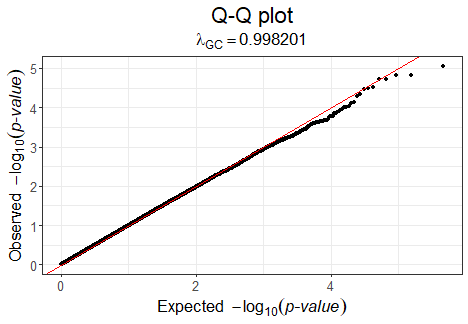
\includegraphics{stats-gene-research-progress-v9_files/figure-latex/unnamed-chunk-2-1.png}

\begin{Shaded}
\begin{Highlighting}[]
\KeywordTok{snp_manhattan}\NormalTok{(}\DataTypeTok{gwas =}\NormalTok{ obj.gwas, }\DataTypeTok{infos.chr =}\NormalTok{ CHR, }\DataTypeTok{infos.pos =}\NormalTok{ POS)}
\end{Highlighting}
\end{Shaded}

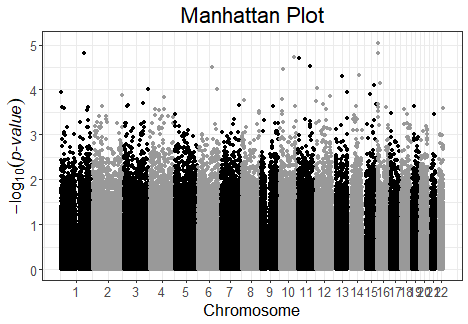
\includegraphics{stats-gene-research-progress-v9_files/figure-latex/unnamed-chunk-2-2.png}

\begin{Shaded}
\begin{Highlighting}[]
\CommentTok{### Histogram of p-values:}
\NormalTok{p_vals <-}\StringTok{ }\DecValTok{2}\OperatorTok{*}\KeywordTok{pnorm}\NormalTok{(}\OperatorTok{-}\KeywordTok{abs}\NormalTok{(obj.gwas}\OperatorTok{$}\NormalTok{score))}
\KeywordTok{hist}\NormalTok{(p_vals, }\DataTypeTok{breaks =} \DecValTok{30}\NormalTok{)}
\end{Highlighting}
\end{Shaded}

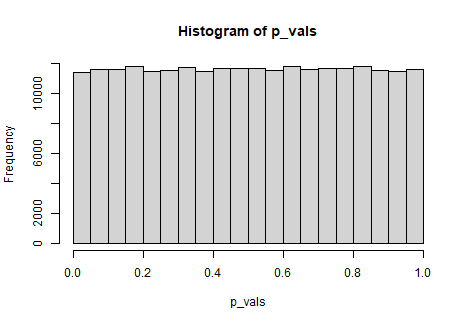
\includegraphics{stats-gene-research-progress-v9_files/figure-latex/unnamed-chunk-2-3.png}

Based on the plots above, we can conclude that p-value's distribution is
very close to the uniform distribution, which is what we expect.

\clearpage

\textbf{Proposed Method: Assuming additive effect}

Then, we will apply our proposed methodology for detection of missing
interaction, assuming the true effect of gene is additive. Again, we
expect to see the distribution of p-values to be close to uniform.

\begin{Shaded}
\begin{Highlighting}[]
\KeywordTok{load}\NormalTok{(}\StringTok{"D:/gwas-practice/additive_testing.Rdata"}\NormalTok{)}

\CommentTok{## View of the result}
\KeywordTok{head}\NormalTok{(result_P1)}
\end{Highlighting}
\end{Shaded}

\begin{verbatim}
## # A tibble: 6 x 5
##   SNP            CHR      BP    stats      P
##   <chr>        <int>   <int>    <dbl>  <dbl>
## 1 SNP1-840643      1  850780 0.000836 0.977 
## 2 SNP1-842827      1  852964 0.0175   0.895 
## 3 SNP1-908480      1  918617 2.39     0.122 
## 4 rs3766192        1 1017197 0.421    0.516 
## 5 rs3766191        1 1017587 4.33     0.0375
## 6 SNP1-1013008     1 1023145 1.41     0.236
\end{verbatim}

\begin{Shaded}
\begin{Highlighting}[]
\CommentTok{## QQ plot of p-values}
\KeywordTok{qq}\NormalTok{(}\KeywordTok{na.omit}\NormalTok{(result_P1}\OperatorTok{$}\NormalTok{P))}
\end{Highlighting}
\end{Shaded}

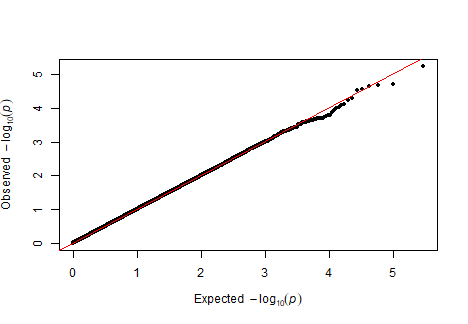
\includegraphics{stats-gene-research-progress-v9_files/figure-latex/unnamed-chunk-3-1.png}

\begin{Shaded}
\begin{Highlighting}[]
\CommentTok{## Manhattan plot of p-values:}
\KeywordTok{manhattan}\NormalTok{(}\KeywordTok{na.omit}\NormalTok{(result_P1), }\DataTypeTok{suggestiveline =}\NormalTok{ F,}\DataTypeTok{genomewideline =} \OperatorTok{-}\KeywordTok{log}\NormalTok{(}\FloatTok{0.05}\OperatorTok{/}\KeywordTok{nrow}\NormalTok{(G)))}
\end{Highlighting}
\end{Shaded}

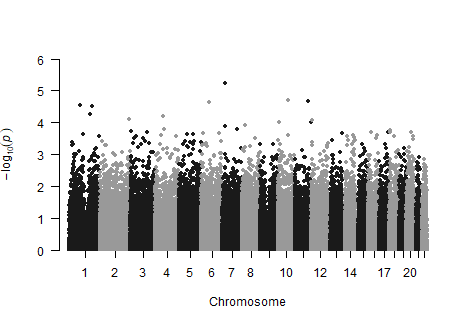
\includegraphics{stats-gene-research-progress-v9_files/figure-latex/unnamed-chunk-3-2.png}

\begin{Shaded}
\begin{Highlighting}[]
\CommentTok{## Histogram of p-values:}
\KeywordTok{hist}\NormalTok{(result_P1}\OperatorTok{$}\NormalTok{P, }\DataTypeTok{breaks =} \DecValTok{30}\NormalTok{)}
\end{Highlighting}
\end{Shaded}

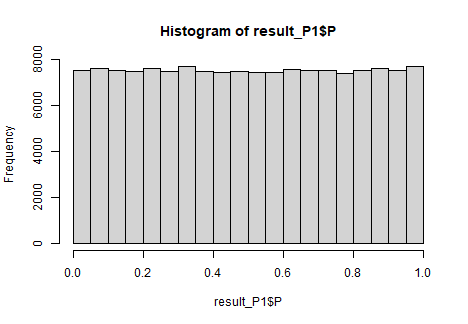
\includegraphics{stats-gene-research-progress-v9_files/figure-latex/unnamed-chunk-3-3.png}

\clearpage

\hypertarget{simulation-to-check-power}{%
\subsection{Simulation to check
power:}\label{simulation-to-check-power}}

In this section, we consider to check the power of our proposed approach
for detecting GxE interaction via two different simulation settings. We
first compare the power of the proposed method with the power of the
oracle method when information of \(E\) can be collected accurately, and
then compare their powers when there is a measurement error in \(E\).
For all of these settings, we assume that there is only one casual gene
in the model, and that true casual gene has both main effect and
interaction effect with \(E\).

\hypertarget{power-of-the-proposed-method}{%
\subsubsection{Power of the proposed
method:}\label{power-of-the-proposed-method}}

In this case, we consider the following model:
\[Y^* = \beta_0 + \beta_GG_k + \beta_EE+\gamma G_kE + \epsilon\]

Here \(G_k\) is the casual gene we randomly sampled from the genome,
with the constraint that \(G_k\) should have MAF at least 0.3. The
values of our parameters are:

\begin{itemize}
\tightlist
\item
  \(\beta_0= -1, \beta_G=0.8, \beta_E= 0.3,\gamma=0.5\)
\item
  \(E \sim N(0,1)\)
\item
  \(\epsilon \sim N(0,0.5)\)
\end{itemize}

\begin{Shaded}
\begin{Highlighting}[]
\CommentTok{############### Power of the proposed method for interaction: With one casual genes}

\CommentTok{### Again, first take account of the linkage disequilibrium problem:}
\KeywordTok{set.seed}\NormalTok{(}\DecValTok{123}\NormalTok{,}\DataTypeTok{sample.kind=}\StringTok{"Rounding"}\NormalTok{)}
\NormalTok{indx <-}\StringTok{ }\DecValTok{1}\OperatorTok{:}\KeywordTok{ncol}\NormalTok{(G)}
\NormalTok{G_using <-}\StringTok{ }\NormalTok{G[,indx]}
\NormalTok{CHR_using <-}\StringTok{ }\NormalTok{CHR[indx]}
\NormalTok{POS_using <-}\StringTok{ }\NormalTok{POS[indx]}


\CommentTok{### Randomly sample 1 genes:}
\NormalTok{p <-}\StringTok{ }\DecValTok{1}
\CommentTok{### Need to make sure that all genotypes have enough frequencies in the selected genes:}
\NormalTok{freq_counts <-}\StringTok{ }\KeywordTok{big_counts}\NormalTok{(G,}\DataTypeTok{ind.col =}\NormalTok{ indx)}
\NormalTok{MAF <-}\StringTok{ }\KeywordTok{snp_MAF}\NormalTok{(G,}\DataTypeTok{ind.col =}\NormalTok{ indx)}
\NormalTok{Qualified <-}\StringTok{ }\NormalTok{freq_counts[}\DecValTok{3}\NormalTok{,] }\OperatorTok{>=}\StringTok{ }\DecValTok{200} \OperatorTok{&}\StringTok{ }\NormalTok{MAF}\OperatorTok{>=}\FloatTok{0.3}
\NormalTok{POS_EFF <-}\StringTok{ }\KeywordTok{sample}\NormalTok{(POS_using[Qualified], }\DataTypeTok{size =} \DecValTok{1}\NormalTok{)}


\CommentTok{### Randomly sample 1/2 genes with strong effects and 1/2 genes with weak effects}
\NormalTok{b0 <-}\StringTok{ }\DecValTok{-1}
\NormalTok{bG <-}\StringTok{ }\FloatTok{0.8}
\NormalTok{bint <-}\StringTok{ }\FloatTok{0.8}
\NormalTok{bE <-}\StringTok{ }\FloatTok{0.3}


\CommentTok{### Generate the underlying environment variable:}
\NormalTok{E <-}\StringTok{ }\KeywordTok{rnorm}\NormalTok{(}\DataTypeTok{n =} \KeywordTok{length}\NormalTok{(G_using[,}\DecValTok{1}\NormalTok{]), }\DataTypeTok{sd =} \DecValTok{1}\NormalTok{)}

\CommentTok{### Generate the latent variable:}
\NormalTok{y_lat <-}\StringTok{ }\NormalTok{b0 }\OperatorTok{+}\StringTok{ }\NormalTok{bG}\OperatorTok{*}\NormalTok{G_using[,POS_using }\OperatorTok{==}\StringTok{ }\NormalTok{POS_EFF] }\OperatorTok{+}\StringTok{ }\NormalTok{bE}\OperatorTok{*}\NormalTok{E }\OperatorTok{+}\StringTok{ }\NormalTok{bint}\OperatorTok{*}\NormalTok{E}\OperatorTok{*}\NormalTok{G_using[,POS_using }\OperatorTok{==}\StringTok{ }\NormalTok{POS_EFF] }\OperatorTok{+}\StringTok{ }\KeywordTok{rnorm}\NormalTok{(}\DataTypeTok{n =} \KeywordTok{length}\NormalTok{(G_using[,}\DecValTok{1}\NormalTok{]), }\DataTypeTok{sd =} \FloatTok{0.5}\NormalTok{)}
\NormalTok{case_new <-}\StringTok{ }\KeywordTok{ifelse}\NormalTok{(y_lat }\OperatorTok{>}\StringTok{ }\DecValTok{0}\NormalTok{, }\DecValTok{1}\NormalTok{, }\DecValTok{0}\NormalTok{)}

\CommentTok{### case_control ratio: }
\KeywordTok{table}\NormalTok{(case_new)}
\end{Highlighting}
\end{Shaded}

\begin{verbatim}
## case_new
##    0    1 
## 1268  481
\end{verbatim}

\begin{Shaded}
\begin{Highlighting}[]
\CommentTok{#### Testing for interaction effect}
\CommentTok{### Assuming additive model: Testing for non-linearity}
\NormalTok{waldstats_P1 <-}\StringTok{ }\KeywordTok{c}\NormalTok{()}
\NormalTok{p_vals_P1 <-}\StringTok{ }\KeywordTok{c}\NormalTok{()}

\ControlFlowTok{for}\NormalTok{ (i }\ControlFlowTok{in} \DecValTok{1}\OperatorTok{:}\KeywordTok{ncol}\NormalTok{(G_using)) \{}
\NormalTok{  Gi <-}\StringTok{ }\NormalTok{G_using[,i]}
  
  \ControlFlowTok{if}\NormalTok{(}\KeywordTok{length}\NormalTok{(}\KeywordTok{unique}\NormalTok{(Gi)) }\OperatorTok{!=}\StringTok{ }\DecValTok{3}\NormalTok{)\{}
\NormalTok{    waldstats_P1[i] <-}\StringTok{ }\DecValTok{0}
\NormalTok{    p_vals_P1[i] <-}\StringTok{ }\DecValTok{-1}
\NormalTok{  \}}
  \ControlFlowTok{else}\NormalTok{\{}
\NormalTok{    modi <-}\StringTok{ }\KeywordTok{glm}\NormalTok{(case_new }\OperatorTok{~}\StringTok{ }\KeywordTok{factor}\NormalTok{(Gi), }\DataTypeTok{family =} \KeywordTok{binomial}\NormalTok{(}\DataTypeTok{link =} \StringTok{"probit"}\NormalTok{))}
\NormalTok{    waldstats_P1[i] <-}\StringTok{ }\KeywordTok{as.numeric}\NormalTok{(}\KeywordTok{wald.test}\NormalTok{(}\KeywordTok{vcov}\NormalTok{(modi)[}\OperatorTok{-}\DecValTok{1}\NormalTok{,}\OperatorTok{-}\DecValTok{1}\NormalTok{], }\DataTypeTok{b =}\NormalTok{ modi}\OperatorTok{$}\NormalTok{coefficients[}\OperatorTok{-}\DecValTok{1}\NormalTok{], }\DataTypeTok{H0 =} \KeywordTok{matrix}\NormalTok{(}\DecValTok{0}\NormalTok{,}\DataTypeTok{nrow =} \DecValTok{1}\NormalTok{,}\DataTypeTok{ncol =} \DecValTok{1}\NormalTok{), }\DataTypeTok{L =} \KeywordTok{matrix}\NormalTok{(}\KeywordTok{c}\NormalTok{(}\DecValTok{2}\NormalTok{,}\OperatorTok{-}\DecValTok{1}\NormalTok{),}\DataTypeTok{nrow =} \DecValTok{1}\NormalTok{))}\OperatorTok{$}\NormalTok{result}\OperatorTok{$}\NormalTok{chi2[}\DecValTok{1}\NormalTok{])}
\NormalTok{    p_vals_P1[i] <-}\StringTok{ }\KeywordTok{as.numeric}\NormalTok{(}\KeywordTok{wald.test}\NormalTok{(}\KeywordTok{vcov}\NormalTok{(modi)[}\OperatorTok{-}\DecValTok{1}\NormalTok{,}\OperatorTok{-}\DecValTok{1}\NormalTok{], }\DataTypeTok{b =}\NormalTok{ modi}\OperatorTok{$}\NormalTok{coefficients[}\OperatorTok{-}\DecValTok{1}\NormalTok{], }\DataTypeTok{H0 =} \KeywordTok{matrix}\NormalTok{(}\DecValTok{0}\NormalTok{,}\DataTypeTok{nrow =} \DecValTok{1}\NormalTok{,}\DataTypeTok{ncol =} \DecValTok{1}\NormalTok{), }\DataTypeTok{L =} \KeywordTok{matrix}\NormalTok{(}\KeywordTok{c}\NormalTok{(}\DecValTok{2}\NormalTok{,}\OperatorTok{-}\DecValTok{1}\NormalTok{),}\DataTypeTok{nrow =} \DecValTok{1}\NormalTok{))}\OperatorTok{$}\NormalTok{result}\OperatorTok{$}\NormalTok{chi2[}\DecValTok{3}\NormalTok{]) }
\NormalTok{  \}}
\NormalTok{\}}

\NormalTok{result_P_INT <-}\StringTok{ }\KeywordTok{tibble}\NormalTok{(}\DataTypeTok{SNP =}\NormalTok{ obj.bigSNP}\OperatorTok{$}\NormalTok{map}\OperatorTok{$}\NormalTok{marker.ID[indx], }\DataTypeTok{CHR =}\NormalTok{ CHR_using, }\DataTypeTok{BP =}\NormalTok{ POS_using , }\DataTypeTok{stats =}\NormalTok{ waldstats_P1, }\DataTypeTok{P =}\NormalTok{ p_vals_P1) }\OperatorTok\StringTok{ }\KeywordTok{filter}\NormalTok{(P }\OperatorTok{>}\StringTok{ }\DecValTok{0}\NormalTok{)}



\CommentTok{### diagnostic plots:}
\KeywordTok{manhattan}\NormalTok{(result_P_INT, }\DataTypeTok{highlight =}\NormalTok{ result_P_INT}\OperatorTok{$}\NormalTok{SNP[}\KeywordTok{which}\NormalTok{(POS_using }\OperatorTok\StringTok{ }\NormalTok{POS_EFF)], }\DataTypeTok{suggestiveline =} \OtherTok{FALSE}\NormalTok{, }\DataTypeTok{genomewideline =} \OperatorTok{-}\KeywordTok{log10}\NormalTok{(}\DecValTok{5} \OperatorTok{*}\StringTok{ }\NormalTok{(}\DecValTok{10} \OperatorTok{^}\StringTok{ }\DecValTok{-8}\NormalTok{)))}
\end{Highlighting}
\end{Shaded}

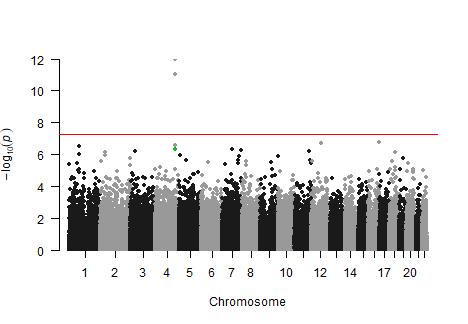
\includegraphics{stats-gene-research-progress-v9_files/figure-latex/OneCasualGene-1.png}

\begin{Shaded}
\begin{Highlighting}[]
\KeywordTok{qq}\NormalTok{(}\KeywordTok{na.omit}\NormalTok{(result_P_INT)}\OperatorTok{$}\NormalTok{P)}
\end{Highlighting}
\end{Shaded}

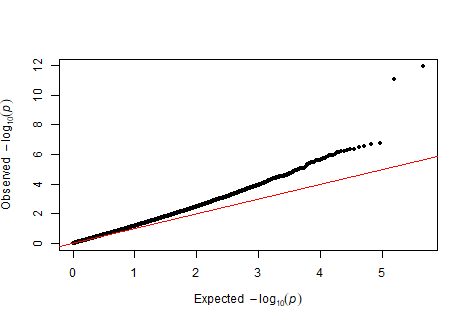
\includegraphics{stats-gene-research-progress-v9_files/figure-latex/OneCasualGene-2.png}

\begin{Shaded}
\begin{Highlighting}[]
\KeywordTok{hist}\NormalTok{(result_P_INT}\OperatorTok{$}\NormalTok{P, }\DataTypeTok{breaks =} \DecValTok{30}\NormalTok{)}
\end{Highlighting}
\end{Shaded}

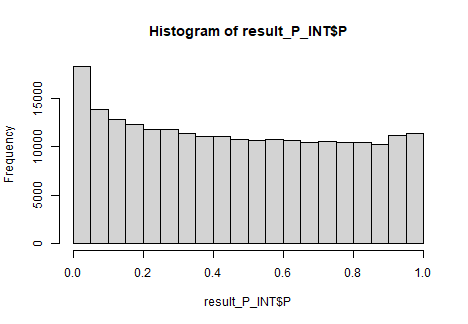
\includegraphics{stats-gene-research-progress-v9_files/figure-latex/OneCasualGene-3.png}

\begin{Shaded}
\begin{Highlighting}[]
\NormalTok{result_P_INT[result_P_INT}\OperatorTok{$}\NormalTok{BP }\OperatorTok\StringTok{ }\NormalTok{POS_EFF, ]}
\end{Highlighting}
\end{Shaded}

\begin{verbatim}
## # A tibble: 1 x 5
##   SNP              CHR        BP stats        P
##   <chr>          <int>     <int> <dbl>    <dbl>
## 1 SNP4-164081321     4 163861871  50.7 1.07e-12
\end{verbatim}

Here we can see that our proposed method works well to identify the true
casual gene in this simulation example. We assumed a quite large
interaction effect compared to the main effect of \(E\), and we assume a
very small variance for \(\sigma_\epsilon^2\) to make sure that the
casual gene will be easy to be found by our method, since our sample
size is very small in this example.

\clearpage

\hypertarget{aggregating-p-values-through-k-repetitions}{%
\subsubsection{Aggregating p-values through k
repetitions:}\label{aggregating-p-values-through-k-repetitions}}

In order to better understand the power of our proposed method, we will
perform the simulation study with only one casual gene and aggregate the
result for K = 50 times:

Here \(G_k\) is the casual gene we randomly sampled from the genome,
with the constraint that \(G_k\) should have MAF at least 0.25. The
values of our parameters are:

\begin{itemize}
\tightlist
\item
  \(\beta_0= -1, \beta_G=0.8, \beta_E= 0.3,\gamma=0.3\)
\item
  \(E \sim N(0,1)\)
\item
  \(\epsilon \sim N(0,0.5)\)
\end{itemize}

\begin{Shaded}
\begin{Highlighting}[]
\CommentTok{### First randomly draw a position:}
\CommentTok{### Again, first take account of the linkage disequilibrium problem:}
\KeywordTok{set.seed}\NormalTok{(}\DecValTok{12345}\NormalTok{,}\DataTypeTok{sample.kind=}\StringTok{"Rounding"}\NormalTok{)}
\NormalTok{p <-}\StringTok{ }\DecValTok{1}
\NormalTok{freq_counts <-}\StringTok{ }\KeywordTok{big_counts}\NormalTok{(G)}
\NormalTok{MAF <-}\StringTok{ }\KeywordTok{snp_MAF}\NormalTok{(G)}
\NormalTok{Qualified <-}\StringTok{ }\NormalTok{freq_counts[}\DecValTok{3}\NormalTok{,] }\OperatorTok{>=}\StringTok{ }\DecValTok{200} \OperatorTok{&}\StringTok{ }\NormalTok{MAF}\OperatorTok{>=}\FloatTok{0.25}
\NormalTok{POS_EFF <-}\StringTok{ }\KeywordTok{sample}\NormalTok{(POS[Qualified], }\DataTypeTok{size =} \DecValTok{1}\NormalTok{)}
\NormalTok{indx <-}\StringTok{ }\KeywordTok{which}\NormalTok{(CHR }\OperatorTok{==}\StringTok{ }\NormalTok{CHR[}\KeywordTok{which}\NormalTok{(POS }\OperatorTok{==}\StringTok{ }\NormalTok{POS_EFF)])}
\NormalTok{G_using <-}\StringTok{ }\NormalTok{G[,indx]}
\NormalTok{CHR_using <-}\StringTok{ }\NormalTok{CHR[indx]}
\NormalTok{POS_using <-}\StringTok{ }\NormalTok{POS[indx]}

\CommentTok{### Let's repeat for 30 times}
\NormalTok{result <-}\StringTok{ }\KeywordTok{Proposed_Aggreg}\NormalTok{(}\DataTypeTok{k =} \DecValTok{10}\NormalTok{, }\DataTypeTok{SNP_names =}\NormalTok{ obj.bigSNP}\OperatorTok{$}\NormalTok{map}\OperatorTok{$}\NormalTok{marker.ID[indx], }\DataTypeTok{Gusing =}\NormalTok{ G_using, }\DataTypeTok{POS_using =}\NormalTok{ POS_using, }\DataTypeTok{CHR_using =}\NormalTok{ CHR_using, }\DataTypeTok{effective_gene =}\NormalTok{ POS_EFF, }\DataTypeTok{bE =} \FloatTok{0.3}\NormalTok{, }\DataTypeTok{bint =} \FloatTok{0.8}\NormalTok{, }\DataTypeTok{bG =} \FloatTok{0.8}\NormalTok{, }\DataTypeTok{sigmaE =} \DecValTok{1}\NormalTok{, }\DataTypeTok{sigma_eps =} \FloatTok{0.5}\NormalTok{)}
\NormalTok{result <-}\StringTok{ }\NormalTok{result }\OperatorTok\StringTok{ }\KeywordTok{filter}\NormalTok{(P }\OperatorTok{>}\StringTok{ }\DecValTok{0}\NormalTok{)}
\KeywordTok{manhattan}\NormalTok{(result, }\DataTypeTok{highlight =}\NormalTok{ obj.bigSNP}\OperatorTok{$}\NormalTok{map}\OperatorTok{$}\NormalTok{marker.ID[indx][}\KeywordTok{which}\NormalTok{(POS_using }\OperatorTok{==}\StringTok{ }\NormalTok{POS_EFF)], }\DataTypeTok{suggestiveline =} \OtherTok{FALSE}\NormalTok{, }\DataTypeTok{genomewideline =} \OperatorTok{-}\KeywordTok{log10}\NormalTok{(}\DecValTok{5} \OperatorTok{*}\StringTok{ }\NormalTok{(}\DecValTok{10} \OperatorTok{^}\StringTok{ }\DecValTok{-8}\NormalTok{)))}
\end{Highlighting}
\end{Shaded}

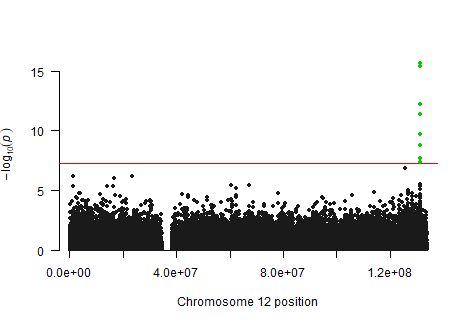
\includegraphics{stats-gene-research-progress-v9_files/figure-latex/Agg-1.png}

\begin{Shaded}
\begin{Highlighting}[]
\KeywordTok{qq}\NormalTok{(}\KeywordTok{na.omit}\NormalTok{(result)}\OperatorTok{$}\NormalTok{P)}
\end{Highlighting}
\end{Shaded}

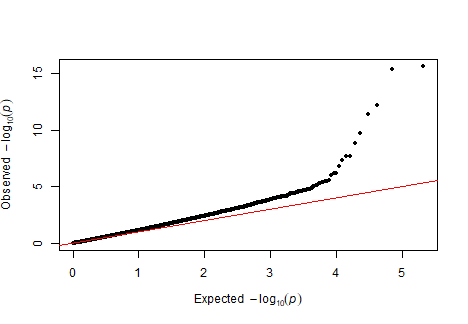
\includegraphics{stats-gene-research-progress-v9_files/figure-latex/Agg-2.png}

\begin{Shaded}
\begin{Highlighting}[]
\KeywordTok{hist}\NormalTok{(result}\OperatorTok{$}\NormalTok{P, }\DataTypeTok{breaks =} \DecValTok{30}\NormalTok{)}
\end{Highlighting}
\end{Shaded}

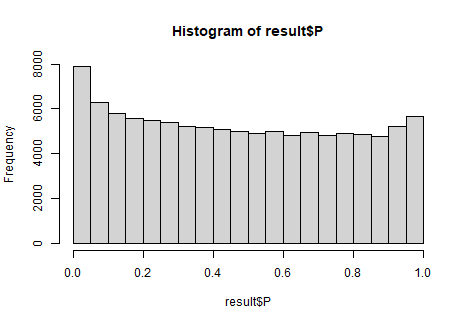
\includegraphics{stats-gene-research-progress-v9_files/figure-latex/Agg-3.png}

\begin{Shaded}
\begin{Highlighting}[]
\CommentTok{### Check for power:}
\NormalTok{classifications <-}\StringTok{ }\NormalTok{result }\OperatorTok\StringTok{ }\KeywordTok{filter}\NormalTok{(BP }\OperatorTok{==}\StringTok{ }\NormalTok{POS_EFF) }\OperatorTok\StringTok{ }\KeywordTok{mutate}\NormalTok{(}\DataTypeTok{classified =} \KeywordTok{ifelse}\NormalTok{(P }\OperatorTok{<=}\StringTok{ }\NormalTok{(}\DecValTok{5} \OperatorTok{*}\StringTok{ }\NormalTok{(}\DecValTok{10} \OperatorTok{^}\StringTok{ }\DecValTok{-8}\NormalTok{)), }\DecValTok{1}\NormalTok{, }\DecValTok{0}\NormalTok{)) }\OperatorTok\StringTok{ }\KeywordTok{select}\NormalTok{(classified) }\OperatorTok\StringTok{ }\KeywordTok{pull}\NormalTok{()}
\KeywordTok{sum}\NormalTok{(classifications)}\OperatorTok{/}\KeywordTok{length}\NormalTok{(classifications)}
\end{Highlighting}
\end{Shaded}

\begin{verbatim}
## [1] 1
\end{verbatim}

\begin{Shaded}
\begin{Highlighting}[]
\CommentTok{### Check for type I error rate:}
\NormalTok{error <-}\StringTok{ }\NormalTok{result }\OperatorTok\StringTok{ }\KeywordTok{filter}\NormalTok{(BP }\OperatorTok{!=}\StringTok{ }\NormalTok{POS_EFF) }\OperatorTok\StringTok{ }\KeywordTok{mutate}\NormalTok{(}\DataTypeTok{classified =} \KeywordTok{ifelse}\NormalTok{(P }\OperatorTok{<=}\StringTok{ }\NormalTok{(}\DecValTok{5} \OperatorTok{*}\StringTok{ }\NormalTok{(}\DecValTok{10} \OperatorTok{^}\StringTok{ }\DecValTok{-8}\NormalTok{)), }\DecValTok{1}\NormalTok{, }\DecValTok{0}\NormalTok{)) }\OperatorTok\StringTok{ }\KeywordTok{select}\NormalTok{(classified) }\OperatorTok\StringTok{ }\KeywordTok{pull}\NormalTok{()}
\KeywordTok{sum}\NormalTok{(error)}\OperatorTok{/}\KeywordTok{length}\NormalTok{(error)}
\end{Highlighting}
\end{Shaded}

\begin{verbatim}
## [1] 0
\end{verbatim}

Based on the result above, with 50 times aggregations, our power is
estimated to be around 10\%, while the type I error rate is estimated to
be zero in these simulations.

Then we changed the setting of our simulation. The values of our
parameters now are:

\begin{itemize}
\tightlist
\item
  \(\beta_0= -1, \beta_G=0.8, \beta_E= 0.3,\gamma=0.5\)
\item
  \(E \sim N(0,1)\)
\item
  \(\epsilon \sim N(0,0.5)\)
\end{itemize}

\begin{Shaded}
\begin{Highlighting}[]
\CommentTok{### First randomly draw a position:}
\CommentTok{### Again, first take account of the linkage disequilibrium problem:}
\KeywordTok{set.seed}\NormalTok{(}\DecValTok{123}\NormalTok{,}\DataTypeTok{sample.kind=}\StringTok{"Rounding"}\NormalTok{)}

\CommentTok{### Let's repeat for 30 times}
\NormalTok{result <-}\StringTok{ }\KeywordTok{Proposed_Aggreg}\NormalTok{(}\DataTypeTok{k =} \DecValTok{50}\NormalTok{, }\DataTypeTok{SNP_names =}\NormalTok{ obj.bigSNP}\OperatorTok{$}\NormalTok{map}\OperatorTok{$}\NormalTok{marker.ID[indx], }\DataTypeTok{Gusing =}\NormalTok{ G_using, }\DataTypeTok{POS_using =}\NormalTok{ POS_using, }\DataTypeTok{CHR_using =}\NormalTok{ CHR_using, }\DataTypeTok{effective_gene =}\NormalTok{ POS_EFF, }\DataTypeTok{bE =} \FloatTok{0.3}\NormalTok{, }\DataTypeTok{bint =} \FloatTok{0.5}\NormalTok{, }\DataTypeTok{bG =} \FloatTok{0.8}\NormalTok{, }\DataTypeTok{sigmaE =} \DecValTok{1}\NormalTok{, }\DataTypeTok{sigma_eps =} \FloatTok{0.5}\NormalTok{)}
\NormalTok{result <-}\StringTok{ }\NormalTok{result }\OperatorTok\StringTok{ }\KeywordTok{filter}\NormalTok{(P }\OperatorTok{>}\StringTok{ }\DecValTok{0}\NormalTok{)}

\KeywordTok{qq}\NormalTok{(}\KeywordTok{na.omit}\NormalTok{(result)}\OperatorTok{$}\NormalTok{P)}
\end{Highlighting}
\end{Shaded}

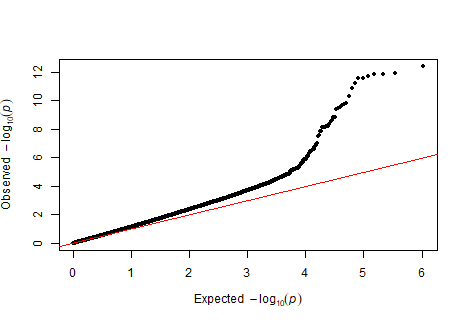
\includegraphics{stats-gene-research-progress-v9_files/figure-latex/unnamed-chunk-4-1.png}

\begin{Shaded}
\begin{Highlighting}[]
\KeywordTok{hist}\NormalTok{(result}\OperatorTok{$}\NormalTok{P, }\DataTypeTok{breaks =} \DecValTok{30}\NormalTok{)}
\end{Highlighting}
\end{Shaded}

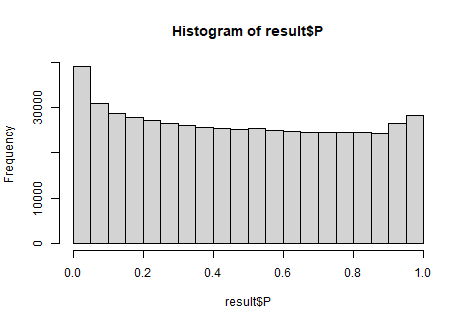
\includegraphics{stats-gene-research-progress-v9_files/figure-latex/unnamed-chunk-4-2.png}

\begin{Shaded}
\begin{Highlighting}[]
\CommentTok{### Check for power:}
\NormalTok{classifications <-}\StringTok{ }\NormalTok{result }\OperatorTok\StringTok{ }\KeywordTok{filter}\NormalTok{(BP }\OperatorTok{==}\StringTok{ }\NormalTok{POS_EFF) }\OperatorTok\StringTok{ }\KeywordTok{mutate}\NormalTok{(}\DataTypeTok{classified =} \KeywordTok{ifelse}\NormalTok{(P }\OperatorTok{<=}\StringTok{ }\NormalTok{(}\DecValTok{5} \OperatorTok{*}\StringTok{ }\NormalTok{(}\DecValTok{10} \OperatorTok{^}\StringTok{ }\DecValTok{-8}\NormalTok{)), }\DecValTok{1}\NormalTok{, }\DecValTok{0}\NormalTok{)) }\OperatorTok\StringTok{ }\KeywordTok{select}\NormalTok{(classified) }\OperatorTok\StringTok{ }\KeywordTok{pull}\NormalTok{()}
\KeywordTok{sum}\NormalTok{(classifications)}\OperatorTok{/}\KeywordTok{length}\NormalTok{(classifications)}
\end{Highlighting}
\end{Shaded}

\begin{verbatim}
## [1] 0.66
\end{verbatim}

\begin{Shaded}
\begin{Highlighting}[]
\CommentTok{### Check for type I error rate:}
\NormalTok{error <-}\StringTok{ }\NormalTok{result }\OperatorTok\StringTok{ }\KeywordTok{filter}\NormalTok{(BP }\OperatorTok{!=}\StringTok{ }\NormalTok{POS_EFF) }\OperatorTok\StringTok{ }\KeywordTok{mutate}\NormalTok{(}\DataTypeTok{classified =} \KeywordTok{ifelse}\NormalTok{(P }\OperatorTok{<=}\StringTok{ }\NormalTok{(}\DecValTok{5} \OperatorTok{*}\StringTok{ }\NormalTok{(}\DecValTok{10} \OperatorTok{^}\StringTok{ }\DecValTok{-8}\NormalTok{)), }\DecValTok{1}\NormalTok{, }\DecValTok{0}\NormalTok{)) }\OperatorTok\StringTok{ }\KeywordTok{select}\NormalTok{(classified) }\OperatorTok\StringTok{ }\KeywordTok{pull}\NormalTok{()}
\KeywordTok{sum}\NormalTok{(error)}\OperatorTok{/}\KeywordTok{length}\NormalTok{(error)}
\end{Highlighting}
\end{Shaded}

\begin{verbatim}
## [1] 0
\end{verbatim}

By increasing \(\gamma\) from \(0.3\) to \(0.5\), we can see that the
power of our proposed approach increases significantly.

\textbf{Summary:} Through simulation study above, we found that the
performance of our proposed approach is highly dependent on the
following:

\begin{itemize}
\tightlist
\item
  How large is \(\gamma\) compared to \(\beta_E\): Increasing
  \(\beta_E\) will significantly decrease the power.
\item
  How large is \(Var(\epsilon)= \sigma^2_\epsilon\): Decreasing this
  will increase the power of our procedure, sometimes by a lot.
\item
  How large is \(|\beta_G|\): Higher \(|\beta_G|\) is also associated
  with higher power.
\end{itemize}

\clearpage

\hypertarget{comparison-between-the-proposed-method-with-oracle-method}{%
\subsection{Comparison between the Proposed method with oracle
method:}\label{comparison-between-the-proposed-method-with-oracle-method}}

Here we still consider the 1kGP dataset which we used in the last
section. The true underlying model of our simulation will be:
\[Y^* = \beta_0 + \beta_GG_k + \beta_EE+\gamma G_kE + \epsilon\] with
the following model specifications:

\begin{itemize}
\tightlist
\item
  \(\beta_0= -1, \beta_G=0.8, \beta_E= 0.3,\gamma=0.5\)
\item
  \(E \sim N(0,1)\)
\item
  \(\epsilon \sim N(0,0.5)\) The \(G_k\) will be sampled for six times,
  with different levels of MAF in each time.
\end{itemize}

We will compare our proposed method with the oracle method, which
assumes that the information about \(E\) can be observed (either with
measurement error or not), so the direct test of \(G\times E\) is
possible. When there exists measurement error in \(E\), we assume that
the observed \(\tilde{E}=E+W\) where
\(W \sim N(0,\sigma_w^2 = 0.25\sigma_E^2)\) is independent of \(E\).

\hypertarget{power-comparison}{%
\subsubsection{Power Comparison:}\label{power-comparison}}

\begin{Shaded}
\begin{Highlighting}[]
\KeywordTok{set.seed}\NormalTok{(}\DecValTok{123}\NormalTok{,}\DataTypeTok{sample.kind=}\StringTok{"Rounding"}\NormalTok{)}

\CommentTok{### Sample three casual genes, corresponding to different MAF}
\NormalTok{freq_counts <-}\StringTok{ }\KeywordTok{big_counts}\NormalTok{(G,}\DataTypeTok{ind.col =}\NormalTok{ indx)}
\NormalTok{MAF <-}\StringTok{ }\KeywordTok{snp_MAF}\NormalTok{(G,}\DataTypeTok{ind.col =}\NormalTok{ indx)}
\NormalTok{Qualified <-}\StringTok{ }\NormalTok{freq_counts[}\DecValTok{3}\NormalTok{,] }\OperatorTok{>=}\StringTok{ }\DecValTok{30} \OperatorTok{&}\StringTok{ }\NormalTok{MAF}\OperatorTok{>=}\FloatTok{0.05} \OperatorTok{&}\StringTok{ }\NormalTok{MAF}\OperatorTok{<=}\FloatTok{0.1}
\NormalTok{POS_EFF1 <-}\StringTok{ }\KeywordTok{sample}\NormalTok{(POS_using[Qualified], }\DataTypeTok{size =} \DecValTok{1}\NormalTok{)}
\NormalTok{Qualified <-}\StringTok{ }\NormalTok{freq_counts[}\DecValTok{3}\NormalTok{,] }\OperatorTok{>=}\StringTok{ }\DecValTok{30} \OperatorTok{&}\StringTok{ }\NormalTok{MAF}\OperatorTok{>=}\FloatTok{0.1} \OperatorTok{&}\StringTok{ }\NormalTok{MAF}\OperatorTok{<=}\FloatTok{0.15}
\NormalTok{POS_EFF2 <-}\StringTok{ }\KeywordTok{sample}\NormalTok{(POS_using[Qualified], }\DataTypeTok{size =} \DecValTok{1}\NormalTok{)}
\NormalTok{Qualified <-}\StringTok{ }\NormalTok{freq_counts[}\DecValTok{3}\NormalTok{,] }\OperatorTok{>=}\StringTok{ }\DecValTok{80} \OperatorTok{&}\StringTok{ }\NormalTok{MAF}\OperatorTok{>=}\FloatTok{0.15} \OperatorTok{&}\StringTok{ }\NormalTok{MAF}\OperatorTok{<=}\FloatTok{0.2}
\NormalTok{POS_EFF3 <-}\StringTok{ }\KeywordTok{sample}\NormalTok{(POS_using[Qualified], }\DataTypeTok{size =} \DecValTok{1}\NormalTok{)}
\NormalTok{Qualified <-}\StringTok{ }\NormalTok{freq_counts[}\DecValTok{3}\NormalTok{,] }\OperatorTok{>=}\StringTok{ }\DecValTok{30} \OperatorTok{&}\StringTok{ }\NormalTok{MAF}\OperatorTok{>=}\FloatTok{0.2} \OperatorTok{&}\StringTok{ }\NormalTok{MAF}\OperatorTok{<=}\FloatTok{0.3}
\NormalTok{POS_EFF4 <-}\StringTok{ }\KeywordTok{sample}\NormalTok{(POS_using[Qualified], }\DataTypeTok{size =} \DecValTok{1}\NormalTok{)}
\NormalTok{Qualified <-}\StringTok{ }\NormalTok{freq_counts[}\DecValTok{3}\NormalTok{,] }\OperatorTok{>=}\StringTok{ }\DecValTok{100} \OperatorTok{&}\StringTok{ }\NormalTok{MAF}\OperatorTok{>=}\FloatTok{0.3} \OperatorTok{&}\StringTok{ }\NormalTok{MAF}\OperatorTok{<=}\FloatTok{0.4}
\NormalTok{POS_EFF5 <-}\StringTok{ }\KeywordTok{sample}\NormalTok{(POS_using[Qualified], }\DataTypeTok{size =} \DecValTok{1}\NormalTok{)}
\NormalTok{Qualified <-}\StringTok{ }\NormalTok{freq_counts[}\DecValTok{3}\NormalTok{,] }\OperatorTok{>=}\StringTok{ }\DecValTok{30} \OperatorTok{&}\StringTok{ }\NormalTok{MAF}\OperatorTok{>=}\FloatTok{0.4}
\NormalTok{POS_EFF6 <-}\StringTok{ }\KeywordTok{sample}\NormalTok{(POS_using[Qualified], }\DataTypeTok{size =} \DecValTok{1}\NormalTok{)}


\CommentTok{### show their corresponding MAF:}
\KeywordTok{sort}\NormalTok{(MAF[POS_using }\OperatorTok\StringTok{ }\KeywordTok{c}\NormalTok{(POS_EFF1,POS_EFF2,POS_EFF3, POS_EFF4, POS_EFF5, POS_EFF6)])}
\end{Highlighting}
\end{Shaded}

\begin{verbatim}
## [1] 0.0703259 0.1143511 0.1795312 0.2307033 0.3807890 0.4885649
\end{verbatim}

\begin{Shaded}
\begin{Highlighting}[]
\CommentTok{### Compute power of each case:}
\KeywordTok{suppressWarnings}\NormalTok{(power1 <-}\StringTok{ }\KeywordTok{Compare_Aggreg_power}\NormalTok{(}\DataTypeTok{k =} \DecValTok{100}\NormalTok{, }\DataTypeTok{G_using =}\NormalTok{ G_using, }\DataTypeTok{POS_using =}\NormalTok{ POS_using, }\DataTypeTok{effective_gene =}\NormalTok{ POS_EFF1, }\DataTypeTok{sigma_eps =} \FloatTok{0.5}\NormalTok{))}
\NormalTok{power1 <-}\StringTok{ }\NormalTok{power1 }\OperatorTok{<=}\StringTok{ }\DecValTok{5} \OperatorTok{*}\StringTok{ }\NormalTok{(}\DecValTok{10} \OperatorTok{^}\StringTok{ }\DecValTok{-8}\NormalTok{)}
\NormalTok{power1 <-}\StringTok{ }\KeywordTok{apply}\NormalTok{(power1, }\DataTypeTok{MARGIN =} \DecValTok{2}\NormalTok{, }\DataTypeTok{FUN =}\NormalTok{ mean)}

\KeywordTok{suppressWarnings}\NormalTok{(power2 <-}\StringTok{ }\KeywordTok{Compare_Aggreg_power}\NormalTok{(}\DataTypeTok{k =} \DecValTok{100}\NormalTok{, }\DataTypeTok{G_using =}\NormalTok{ G_using, }\DataTypeTok{POS_using =}\NormalTok{ POS_using, }\DataTypeTok{effective_gene =}\NormalTok{ POS_EFF2, }\DataTypeTok{sigma_eps =} \FloatTok{0.5}\NormalTok{))}
\NormalTok{power2 <-}\StringTok{ }\NormalTok{power2 }\OperatorTok{<=}\StringTok{ }\DecValTok{5} \OperatorTok{*}\StringTok{ }\NormalTok{(}\DecValTok{10} \OperatorTok{^}\StringTok{ }\DecValTok{-8}\NormalTok{)}
\NormalTok{power2 <-}\StringTok{ }\KeywordTok{apply}\NormalTok{(power2, }\DataTypeTok{MARGIN =} \DecValTok{2}\NormalTok{, }\DataTypeTok{FUN =}\NormalTok{ mean)}

\KeywordTok{suppressWarnings}\NormalTok{(power3 <-}\StringTok{ }\KeywordTok{Compare_Aggreg_power}\NormalTok{(}\DataTypeTok{k =} \DecValTok{100}\NormalTok{, }\DataTypeTok{G_using =}\NormalTok{ G_using, }\DataTypeTok{POS_using =}\NormalTok{ POS_using, }\DataTypeTok{effective_gene =}\NormalTok{ POS_EFF3, }\DataTypeTok{sigma_eps =} \FloatTok{0.5}\NormalTok{))}
\NormalTok{power3 <-}\StringTok{ }\NormalTok{power3 }\OperatorTok{<=}\StringTok{ }\DecValTok{5} \OperatorTok{*}\StringTok{ }\NormalTok{(}\DecValTok{10} \OperatorTok{^}\StringTok{ }\DecValTok{-8}\NormalTok{)}
\NormalTok{power3 <-}\StringTok{ }\KeywordTok{apply}\NormalTok{(power3, }\DataTypeTok{MARGIN =} \DecValTok{2}\NormalTok{, }\DataTypeTok{FUN =}\NormalTok{ mean)}

\KeywordTok{suppressWarnings}\NormalTok{(power4 <-}\StringTok{ }\KeywordTok{Compare_Aggreg_power}\NormalTok{(}\DataTypeTok{k =} \DecValTok{100}\NormalTok{, }\DataTypeTok{G_using =}\NormalTok{ G_using, }\DataTypeTok{POS_using =}\NormalTok{ POS_using, }\DataTypeTok{effective_gene =}\NormalTok{ POS_EFF4, }\DataTypeTok{sigma_eps =} \FloatTok{0.5}\NormalTok{))}
\NormalTok{power4 <-}\StringTok{ }\NormalTok{power4 }\OperatorTok{<=}\StringTok{ }\DecValTok{5} \OperatorTok{*}\StringTok{ }\NormalTok{(}\DecValTok{10} \OperatorTok{^}\StringTok{ }\DecValTok{-8}\NormalTok{)}
\NormalTok{power4 <-}\StringTok{ }\KeywordTok{apply}\NormalTok{(power4, }\DataTypeTok{MARGIN =} \DecValTok{2}\NormalTok{, }\DataTypeTok{FUN =}\NormalTok{ mean)}

\KeywordTok{suppressWarnings}\NormalTok{(power5 <-}\StringTok{ }\KeywordTok{Compare_Aggreg_power}\NormalTok{(}\DataTypeTok{k =} \DecValTok{100}\NormalTok{, }\DataTypeTok{G_using =}\NormalTok{ G_using, }\DataTypeTok{POS_using =}\NormalTok{ POS_using, }\DataTypeTok{effective_gene =}\NormalTok{ POS_EFF5, }\DataTypeTok{sigma_eps =} \FloatTok{0.5}\NormalTok{))}
\NormalTok{power5 <-}\StringTok{ }\NormalTok{power5 }\OperatorTok{<=}\StringTok{ }\DecValTok{5} \OperatorTok{*}\StringTok{ }\NormalTok{(}\DecValTok{10} \OperatorTok{^}\StringTok{ }\DecValTok{-8}\NormalTok{)}
\NormalTok{power5 <-}\StringTok{ }\KeywordTok{apply}\NormalTok{(power5, }\DataTypeTok{MARGIN =} \DecValTok{2}\NormalTok{, }\DataTypeTok{FUN =}\NormalTok{ mean)}

\KeywordTok{suppressWarnings}\NormalTok{(power6 <-}\StringTok{ }\KeywordTok{Compare_Aggreg_power}\NormalTok{(}\DataTypeTok{k =} \DecValTok{100}\NormalTok{, }\DataTypeTok{G_using =}\NormalTok{ G_using, }\DataTypeTok{POS_using =}\NormalTok{ POS_using, }\DataTypeTok{effective_gene =}\NormalTok{ POS_EFF6, }\DataTypeTok{sigma_eps =} \FloatTok{0.5}\NormalTok{))}
\NormalTok{power6 <-}\StringTok{ }\NormalTok{power6 }\OperatorTok{<=}\StringTok{ }\DecValTok{5} \OperatorTok{*}\StringTok{ }\NormalTok{(}\DecValTok{10} \OperatorTok{^}\StringTok{ }\DecValTok{-8}\NormalTok{)}
\NormalTok{power6 <-}\StringTok{ }\KeywordTok{apply}\NormalTok{(power6, }\DataTypeTok{MARGIN =} \DecValTok{2}\NormalTok{, }\DataTypeTok{FUN =}\NormalTok{ mean)}
\CommentTok{## Table:}
\NormalTok{power <-}\StringTok{ }\KeywordTok{as_tibble}\NormalTok{(}\KeywordTok{as.matrix}\NormalTok{(}\KeywordTok{rbind}\NormalTok{(power1,power2,power3, power4,power5,power6))) }\OperatorTok\StringTok{ }\KeywordTok{mutate}\NormalTok{(}\DataTypeTok{MAF =} \KeywordTok{sort}\NormalTok{(MAF[POS_using }\OperatorTok\StringTok{ }\KeywordTok{c}\NormalTok{(POS_EFF1,POS_EFF2,POS_EFF3,POS_EFF4,POS_EFF5,POS_EFF6)]))}
\NormalTok{kableExtra}\OperatorTok{::}\KeywordTok{kable}\NormalTok{(power,}\DataTypeTok{caption =} \StringTok{"Comparison of Power"}\NormalTok{)}
\end{Highlighting}
\end{Shaded}

\begin{table}

\caption{\label{tab:PowerComparison}Comparison of Power}
\centering
\begin{tabular}[t]{r|r|r|r}
\hline
proposed & oracle & oracle\_error & MAF\\
\hline
0.00 & 0.54 & 0.12 & 0.0703259\\
\hline
0.02 & 0.97 & 0.50 & 0.1143511\\
\hline
0.14 & 1.00 & 0.95 & 0.1795312\\
\hline
0.36 & 1.00 & 0.99 & 0.2307033\\
\hline
0.70 & 1.00 & 1.00 & 0.3807890\\
\hline
0.70 & 1.00 & 1.00 & 0.4885649\\
\hline
\end{tabular}
\end{table}

\begin{Shaded}
\begin{Highlighting}[]
\CommentTok{## Figure:}
\NormalTok{power_plot <-}\StringTok{ }\NormalTok{power }\OperatorTok\StringTok{ }\KeywordTok{pivot_longer}\NormalTok{(proposed}\OperatorTok{:}\NormalTok{oracle_error, }\StringTok{"Type"}\NormalTok{, }\DataTypeTok{values_to =} \StringTok{"Power"}\NormalTok{) }\OperatorTok\StringTok{ }\KeywordTok{mutate}\NormalTok{(}\DataTypeTok{Type =} \KeywordTok{factor}\NormalTok{(Type))}
\KeywordTok{levels}\NormalTok{(power_plot}\OperatorTok{$}\NormalTok{Type) <-}\StringTok{ }\KeywordTok{c}\NormalTok{(}\StringTok{"with_E"}\NormalTok{,}\StringTok{"with_E_error"}\NormalTok{, }\StringTok{"without_E"}\NormalTok{)}
\NormalTok{power_plot }\OperatorTok\StringTok{ }\KeywordTok{ggplot}\NormalTok{(}\KeywordTok{aes}\NormalTok{(MAF,Power,}\DataTypeTok{color =}\NormalTok{ Type)) }\OperatorTok{+}\StringTok{ }\KeywordTok{geom_line}\NormalTok{()}
\end{Highlighting}
\end{Shaded}

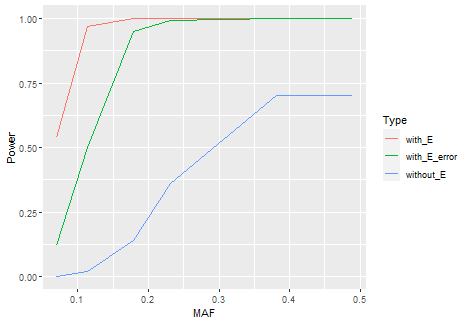
\includegraphics{stats-gene-research-progress-v9_files/figure-latex/PowerComparison-1.png}

Seems like the oracle method with information of \texttt{E} will have
better power than the proposed method, regardless whether there is
measurement error. This difference gets smaller as \texttt{MAF}
increases.

\clearpage

\hypertarget{type-i-error-comparison}{%
\subsubsection{Type I error Comparison:}\label{type-i-error-comparison}}

\begin{Shaded}
\begin{Highlighting}[]
\KeywordTok{set.seed}\NormalTok{(}\DecValTok{123}\NormalTok{,}\DataTypeTok{sample.kind=}\StringTok{"Rounding"}\NormalTok{)}

\CommentTok{### Sample three casual genes, corresponding to different MAF}
\NormalTok{freq_counts <-}\StringTok{ }\KeywordTok{big_counts}\NormalTok{(G,}\DataTypeTok{ind.col =}\NormalTok{ indx)}
\NormalTok{MAF <-}\StringTok{ }\KeywordTok{snp_MAF}\NormalTok{(G,}\DataTypeTok{ind.col =}\NormalTok{ indx)}
\NormalTok{Qualified <-}\StringTok{ }\NormalTok{freq_counts[}\DecValTok{3}\NormalTok{,] }\OperatorTok{>=}\StringTok{ }\DecValTok{30} \OperatorTok{&}\StringTok{ }\NormalTok{MAF}\OperatorTok{>=}\FloatTok{0.05} \OperatorTok{&}\StringTok{ }\NormalTok{MAF}\OperatorTok{<=}\FloatTok{0.1}
\NormalTok{POS_EFF1 <-}\StringTok{ }\KeywordTok{sample}\NormalTok{(POS_using[Qualified], }\DataTypeTok{size =} \DecValTok{1}\NormalTok{)}
\NormalTok{Qualified <-}\StringTok{ }\NormalTok{freq_counts[}\DecValTok{3}\NormalTok{,] }\OperatorTok{>=}\StringTok{ }\DecValTok{80} \OperatorTok{&}\StringTok{ }\NormalTok{MAF}\OperatorTok{>=}\FloatTok{0.1} \OperatorTok{&}\StringTok{ }\NormalTok{MAF}\OperatorTok{<=}\FloatTok{0.15}
\NormalTok{POS_EFF2 <-}\StringTok{ }\KeywordTok{sample}\NormalTok{(POS_using[Qualified], }\DataTypeTok{size =} \DecValTok{1}\NormalTok{)}
\NormalTok{Qualified <-}\StringTok{ }\NormalTok{freq_counts[}\DecValTok{3}\NormalTok{,] }\OperatorTok{>=}\StringTok{ }\DecValTok{100} \OperatorTok{&}\StringTok{ }\NormalTok{MAF}\OperatorTok{>=}\FloatTok{0.15} \OperatorTok{&}\StringTok{ }\NormalTok{MAF}\OperatorTok{<=}\FloatTok{0.2}
\NormalTok{POS_EFF3 <-}\StringTok{ }\KeywordTok{sample}\NormalTok{(POS_using[Qualified], }\DataTypeTok{size =} \DecValTok{1}\NormalTok{)}
\NormalTok{Qualified <-}\StringTok{ }\NormalTok{freq_counts[}\DecValTok{3}\NormalTok{,] }\OperatorTok{>=}\StringTok{ }\DecValTok{100} \OperatorTok{&}\StringTok{ }\NormalTok{MAF}\OperatorTok{>=}\FloatTok{0.2} \OperatorTok{&}\StringTok{ }\NormalTok{MAF}\OperatorTok{<=}\FloatTok{0.25}
\NormalTok{POS_EFF4 <-}\StringTok{ }\KeywordTok{sample}\NormalTok{(POS_using[Qualified], }\DataTypeTok{size =} \DecValTok{1}\NormalTok{)}
\NormalTok{Qualified <-}\StringTok{ }\NormalTok{freq_counts[}\DecValTok{3}\NormalTok{,] }\OperatorTok{>=}\StringTok{ }\DecValTok{100} \OperatorTok{&}\StringTok{ }\NormalTok{MAF}\OperatorTok{>=}\FloatTok{0.25} \OperatorTok{&}\StringTok{ }\NormalTok{MAF}\OperatorTok{<=}\FloatTok{0.3}
\NormalTok{POS_EFF5 <-}\StringTok{ }\KeywordTok{sample}\NormalTok{(POS_using[Qualified], }\DataTypeTok{size =} \DecValTok{1}\NormalTok{)}
\NormalTok{Qualified <-}\StringTok{ }\NormalTok{freq_counts[}\DecValTok{3}\NormalTok{,] }\OperatorTok{>=}\StringTok{ }\DecValTok{100} \OperatorTok{&}\StringTok{ }\NormalTok{MAF}\OperatorTok{>=}\FloatTok{0.3}
\NormalTok{POS_EFF6 <-}\StringTok{ }\KeywordTok{sample}\NormalTok{(POS_using[Qualified], }\DataTypeTok{size =} \DecValTok{1}\NormalTok{)}
\CommentTok{### show their corresponding MAF:}
\KeywordTok{sort}\NormalTok{(MAF[POS_using }\OperatorTok\StringTok{ }\KeywordTok{c}\NormalTok{(POS_EFF1,POS_EFF2,POS_EFF3,POS_EFF4,POS_EFF5,POS_EFF6)])}
\end{Highlighting}
\end{Shaded}

\begin{verbatim}
## [1] 0.0703259 0.1477987 0.1975415 0.2135506 0.2695826 0.4885649
\end{verbatim}

\begin{Shaded}
\begin{Highlighting}[]
\CommentTok{### Compute type I error rate of each case:}
\CommentTok{#1:}
\NormalTok{error1 <-}\StringTok{ }\KeywordTok{Compare_Aggreg_power}\NormalTok{(}\DataTypeTok{k =} \DecValTok{2000}\NormalTok{, }\DataTypeTok{G_using =}\NormalTok{ G_using, }\DataTypeTok{POS_using =}\NormalTok{ POS_using, }\DataTypeTok{effective_gene =}\NormalTok{ POS_EFF1, }\DataTypeTok{b0 =} \DecValTok{-1}\NormalTok{,}\DataTypeTok{bE =} \FloatTok{0.3}\NormalTok{, }\DataTypeTok{bG =} \FloatTok{0.8}\NormalTok{, }\DataTypeTok{bint1 =} \DecValTok{0}\NormalTok{, }\DataTypeTok{sigmaE =} \DecValTok{1}\NormalTok{,}\DataTypeTok{sigma_eps =} \DecValTok{1}\NormalTok{, }\DataTypeTok{measure_error_percentage =} \DecValTok{1}\OperatorTok{/}\DecValTok{4}\NormalTok{)}
\NormalTok{r1 <-}\StringTok{ }\NormalTok{error1 }\OperatorTok\StringTok{ }\KeywordTok{summarise}\NormalTok{(}\DataTypeTok{proposed =} \KeywordTok{mean}\NormalTok{(proposed }\OperatorTok{<=}\FloatTok{0.05}\NormalTok{), }\DataTypeTok{oracle =} \KeywordTok{mean}\NormalTok{(oracle }\OperatorTok{<=}\StringTok{ }\FloatTok{0.05}\NormalTok{), }\DataTypeTok{oracle_error =} \KeywordTok{mean}\NormalTok{(oracle_error}\OperatorTok{<=}\StringTok{ }\FloatTok{0.05}\NormalTok{))}



\CommentTok{#2:}
\NormalTok{error2 <-}\StringTok{ }\KeywordTok{Compare_Aggreg_power}\NormalTok{(}\DataTypeTok{k =} \DecValTok{2000}\NormalTok{, }\DataTypeTok{G_using =}\NormalTok{ G_using, }\DataTypeTok{POS_using =}\NormalTok{ POS_using, }\DataTypeTok{effective_gene =}\NormalTok{ POS_EFF2, }\DataTypeTok{b0 =} \DecValTok{-1}\NormalTok{,}\DataTypeTok{bE =} \FloatTok{0.3}\NormalTok{, }\DataTypeTok{bG =} \FloatTok{0.8}\NormalTok{, }\DataTypeTok{bint1 =} \DecValTok{0}\NormalTok{, }\DataTypeTok{sigmaE =} \DecValTok{1}\NormalTok{,}\DataTypeTok{sigma_eps =} \DecValTok{1}\NormalTok{, }\DataTypeTok{measure_error_percentage =} \DecValTok{1}\OperatorTok{/}\DecValTok{4}\NormalTok{)}
\NormalTok{r2 <-}\StringTok{ }\NormalTok{error2 }\OperatorTok\StringTok{ }\KeywordTok{summarise}\NormalTok{(}\DataTypeTok{proposed =} \KeywordTok{mean}\NormalTok{(proposed }\OperatorTok{<=}\FloatTok{0.05}\NormalTok{), }\DataTypeTok{oracle =} \KeywordTok{mean}\NormalTok{(oracle }\OperatorTok{<=}\StringTok{ }\FloatTok{0.05}\NormalTok{), }\DataTypeTok{oracle_error =} \KeywordTok{mean}\NormalTok{(oracle_error}\OperatorTok{<=}\StringTok{ }\FloatTok{0.05}\NormalTok{))}


\CommentTok{#3:}
\NormalTok{error3 <-}\StringTok{ }\KeywordTok{Compare_Aggreg_power}\NormalTok{(}\DataTypeTok{k =} \DecValTok{2000}\NormalTok{, }\DataTypeTok{G_using =}\NormalTok{ G_using, }\DataTypeTok{POS_using =}\NormalTok{ POS_using, }\DataTypeTok{effective_gene =}\NormalTok{ POS_EFF3, }\DataTypeTok{b0 =} \DecValTok{-1}\NormalTok{,}\DataTypeTok{bE =} \FloatTok{0.3}\NormalTok{, }\DataTypeTok{bG =} \FloatTok{0.8}\NormalTok{, }\DataTypeTok{bint1 =} \DecValTok{0}\NormalTok{, }\DataTypeTok{sigmaE =} \DecValTok{1}\NormalTok{,}\DataTypeTok{sigma_eps =} \DecValTok{1}\NormalTok{, }\DataTypeTok{measure_error_percentage =} \DecValTok{1}\OperatorTok{/}\DecValTok{4}\NormalTok{)}
\NormalTok{r3 <-}\StringTok{ }\NormalTok{error3 }\OperatorTok\StringTok{ }\KeywordTok{summarise}\NormalTok{(}\DataTypeTok{proposed =} \KeywordTok{mean}\NormalTok{(proposed }\OperatorTok{<=}\FloatTok{0.05}\NormalTok{), }\DataTypeTok{oracle =} \KeywordTok{mean}\NormalTok{(oracle }\OperatorTok{<=}\StringTok{ }\FloatTok{0.05}\NormalTok{), }\DataTypeTok{oracle_error =} \KeywordTok{mean}\NormalTok{(oracle_error}\OperatorTok{<=}\StringTok{ }\FloatTok{0.05}\NormalTok{))}

\CommentTok{#4:}
\NormalTok{error4 <-}\StringTok{ }\KeywordTok{Compare_Aggreg_power}\NormalTok{(}\DataTypeTok{k =} \DecValTok{2000}\NormalTok{, }\DataTypeTok{G_using =}\NormalTok{ G_using, }\DataTypeTok{POS_using =}\NormalTok{ POS_using, }\DataTypeTok{effective_gene =}\NormalTok{ POS_EFF4, }\DataTypeTok{b0 =} \DecValTok{-1}\NormalTok{,}\DataTypeTok{bE =} \FloatTok{0.3}\NormalTok{, }\DataTypeTok{bG =} \FloatTok{0.8}\NormalTok{, }\DataTypeTok{bint1 =} \DecValTok{0}\NormalTok{, }\DataTypeTok{sigmaE =} \DecValTok{1}\NormalTok{,}\DataTypeTok{sigma_eps =} \DecValTok{1}\NormalTok{, }\DataTypeTok{measure_error_percentage =} \DecValTok{1}\OperatorTok{/}\DecValTok{4}\NormalTok{)}
\NormalTok{r4 <-}\StringTok{ }\NormalTok{error4 }\OperatorTok\StringTok{ }\KeywordTok{summarise}\NormalTok{(}\DataTypeTok{proposed =} \KeywordTok{mean}\NormalTok{(proposed }\OperatorTok{<=}\FloatTok{0.05}\NormalTok{), }\DataTypeTok{oracle =} \KeywordTok{mean}\NormalTok{(oracle }\OperatorTok{<=}\StringTok{ }\FloatTok{0.05}\NormalTok{), }\DataTypeTok{oracle_error =} \KeywordTok{mean}\NormalTok{(oracle_error}\OperatorTok{<=}\StringTok{ }\FloatTok{0.05}\NormalTok{))}



\CommentTok{#5:}
\NormalTok{error5 <-}\StringTok{ }\KeywordTok{Compare_Aggreg_power}\NormalTok{(}\DataTypeTok{k =} \DecValTok{2000}\NormalTok{, }\DataTypeTok{G_using =}\NormalTok{ G_using, }\DataTypeTok{POS_using =}\NormalTok{ POS_using, }\DataTypeTok{effective_gene =}\NormalTok{ POS_EFF5, }\DataTypeTok{b0 =} \DecValTok{-1}\NormalTok{,}\DataTypeTok{bE =} \FloatTok{0.3}\NormalTok{, }\DataTypeTok{bG =} \FloatTok{0.8}\NormalTok{, }\DataTypeTok{bint1 =} \DecValTok{0}\NormalTok{, }\DataTypeTok{sigmaE =} \DecValTok{1}\NormalTok{,}\DataTypeTok{sigma_eps =} \DecValTok{1}\NormalTok{, }\DataTypeTok{measure_error_percentage =} \DecValTok{1}\OperatorTok{/}\DecValTok{4}\NormalTok{)}
\NormalTok{r5 <-}\StringTok{ }\NormalTok{error5 }\OperatorTok\StringTok{ }\KeywordTok{summarise}\NormalTok{(}\DataTypeTok{proposed =} \KeywordTok{mean}\NormalTok{(proposed }\OperatorTok{<=}\FloatTok{0.05}\NormalTok{), }\DataTypeTok{oracle =} \KeywordTok{mean}\NormalTok{(oracle }\OperatorTok{<=}\StringTok{ }\FloatTok{0.05}\NormalTok{), }\DataTypeTok{oracle_error =} \KeywordTok{mean}\NormalTok{(oracle_error}\OperatorTok{<=}\StringTok{ }\FloatTok{0.05}\NormalTok{))}


\CommentTok{#6:}
\NormalTok{error6 <-}\StringTok{ }\KeywordTok{Compare_Aggreg_power}\NormalTok{(}\DataTypeTok{k =} \DecValTok{2000}\NormalTok{, }\DataTypeTok{G_using =}\NormalTok{ G_using, }\DataTypeTok{POS_using =}\NormalTok{ POS_using, }\DataTypeTok{effective_gene =}\NormalTok{ POS_EFF6, }\DataTypeTok{b0 =} \DecValTok{-1}\NormalTok{,}\DataTypeTok{bE =} \FloatTok{0.3}\NormalTok{, }\DataTypeTok{bG =} \FloatTok{0.8}\NormalTok{, }\DataTypeTok{bint1 =} \DecValTok{0}\NormalTok{, }\DataTypeTok{sigmaE =} \DecValTok{1}\NormalTok{,}\DataTypeTok{sigma_eps =} \DecValTok{1}\NormalTok{, }\DataTypeTok{measure_error_percentage =} \DecValTok{1}\OperatorTok{/}\DecValTok{4}\NormalTok{)}
\NormalTok{r6 <-}\StringTok{ }\NormalTok{error6 }\OperatorTok\StringTok{ }\KeywordTok{summarise}\NormalTok{(}\DataTypeTok{proposed =} \KeywordTok{mean}\NormalTok{(proposed }\OperatorTok{<=}\FloatTok{0.05}\NormalTok{), }\DataTypeTok{oracle =} \KeywordTok{mean}\NormalTok{(oracle }\OperatorTok{<=}\StringTok{ }\FloatTok{0.05}\NormalTok{), }\DataTypeTok{oracle_error =} \KeywordTok{mean}\NormalTok{(oracle_error}\OperatorTok{<=}\StringTok{ }\FloatTok{0.05}\NormalTok{))}



\NormalTok{r <-}\StringTok{ }\KeywordTok{as_tibble}\NormalTok{(}\KeywordTok{rbind}\NormalTok{(r1,r2,r3,r4,r5,r6))}
\NormalTok{r}\OperatorTok{$}\NormalTok{MAF <-}\StringTok{ }\KeywordTok{sort}\NormalTok{(MAF[POS_using }\OperatorTok\StringTok{ }\KeywordTok{c}\NormalTok{(POS_EFF1,POS_EFF2,POS_EFF3,POS_EFF4,POS_EFF5,POS_EFF6)])}
\NormalTok{r_plot <-}\StringTok{ }\NormalTok{r }\OperatorTok\StringTok{ }\KeywordTok{rename}\NormalTok{(}\KeywordTok{c}\NormalTok{(}\StringTok{"proposed"}\NormalTok{ =}\StringTok{ "proposed"}\NormalTok{,}\StringTok{"oracle"}\NormalTok{ =}\StringTok{ "oracle"}\NormalTok{)) }\OperatorTok\StringTok{ }\KeywordTok{pivot_longer}\NormalTok{(proposed}\OperatorTok{:}\NormalTok{oracle_error, }\StringTok{"Type"}\NormalTok{, }\DataTypeTok{values_to =} \StringTok{"Error"}\NormalTok{) }\OperatorTok\StringTok{ }\KeywordTok{mutate}\NormalTok{(}\DataTypeTok{Type =} \KeywordTok{factor}\NormalTok{(Type))}
\KeywordTok{levels}\NormalTok{(r_plot}\OperatorTok{$}\NormalTok{Type) <-}\StringTok{ }\KeywordTok{c}\NormalTok{(}\StringTok{"with_E"}\NormalTok{,}\StringTok{"with_E_error"}\NormalTok{, }\StringTok{"without_E"}\NormalTok{)}
\NormalTok{r_plot }\OperatorTok\StringTok{ }\KeywordTok{ggplot}\NormalTok{(}\KeywordTok{aes}\NormalTok{(MAF,Error,}\DataTypeTok{color =}\NormalTok{ Type)) }\OperatorTok{+}\StringTok{ }\KeywordTok{geom_line}\NormalTok{() }\OperatorTok{+}\StringTok{ }\KeywordTok{ylab}\NormalTok{(}\StringTok{"Type I Error"}\NormalTok{) }\OperatorTok{+}\StringTok{ }\KeywordTok{geom_hline}\NormalTok{(}\KeywordTok{aes}\NormalTok{(}\DataTypeTok{yintercept =} \FloatTok{0.05}\NormalTok{))}
\end{Highlighting}
\end{Shaded}

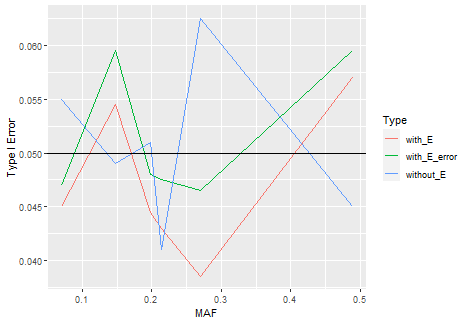
\includegraphics{stats-gene-research-progress-v9_files/figure-latex/errorcompare-1.png}

The above plot shows the relationship between the observed type I error
rate (assuming significance level of 5 percent) with the MAF of the
\texttt{casual} gene in the underlying model. Next, we can take a look
into the relationship between MAF (of non-casual genes) and the observed
type I error rate:

\begin{Shaded}
\begin{Highlighting}[]
\NormalTok{all_error <-}\StringTok{ }\NormalTok{r}
\NormalTok{all_error}\OperatorTok{$}\NormalTok{MAF_level <-}\StringTok{ }\KeywordTok{ifelse}\NormalTok{(all_error}\OperatorTok{$}\NormalTok{MAF }\OperatorTok{>=}\StringTok{ }\FloatTok{0.1}\NormalTok{, }\StringTok{"0.1-0.15"}\NormalTok{,}\StringTok{"0.05-0.1"}\NormalTok{)}
\NormalTok{all_error}\OperatorTok{$}\NormalTok{MAF_level <-}\StringTok{ }\KeywordTok{ifelse}\NormalTok{(all_error}\OperatorTok{$}\NormalTok{MAF }\OperatorTok{>=}\StringTok{ }\FloatTok{0.15}\NormalTok{, }\StringTok{"0.15-0.2"}\NormalTok{, all_error}\OperatorTok{$}\NormalTok{MAF_level)}
\NormalTok{all_error}\OperatorTok{$}\NormalTok{MAF_level <-}\StringTok{ }\KeywordTok{ifelse}\NormalTok{(all_error}\OperatorTok{$}\NormalTok{MAF }\OperatorTok{>=}\StringTok{ }\FloatTok{0.2}\NormalTok{, }\StringTok{"0.2-0.25"}\NormalTok{, all_error}\OperatorTok{$}\NormalTok{MAF_level)}
\NormalTok{all_error}\OperatorTok{$}\NormalTok{MAF_level <-}\StringTok{ }\KeywordTok{ifelse}\NormalTok{(all_error}\OperatorTok{$}\NormalTok{MAF }\OperatorTok{>=}\StringTok{ }\FloatTok{0.25}\NormalTok{, }\StringTok{"0.25-0.3"}\NormalTok{, all_error}\OperatorTok{$}\NormalTok{MAF_level)}
\NormalTok{all_error}\OperatorTok{$}\NormalTok{MAF_level <-}\StringTok{ }\KeywordTok{ifelse}\NormalTok{(all_error}\OperatorTok{$}\NormalTok{MAF }\OperatorTok{>=}\StringTok{ }\FloatTok{0.3}\NormalTok{, }\StringTok{"0.3-0.5"}\NormalTok{, all_error}\OperatorTok{$}\NormalTok{MAF_level)}


\NormalTok{all_error <-}\StringTok{ }\NormalTok{all_error }\OperatorTok\StringTok{ }\KeywordTok{group_by}\NormalTok{(MAF_level) }\OperatorTok\StringTok{ }\KeywordTok{summarise}\NormalTok{(}\DataTypeTok{proposed =} \KeywordTok{mean}\NormalTok{(proposed), }\DataTypeTok{oracle =} \KeywordTok{mean}\NormalTok{(oracle), }\DataTypeTok{oracle_error =} \KeywordTok{mean}\NormalTok{(oracle_error), }\DataTypeTok{number =} \DecValTok{2000}\OperatorTok{*}\KeywordTok{n}\NormalTok{())}

\NormalTok{all_error <-}\StringTok{ }\NormalTok{all_error }\OperatorTok\StringTok{ }\KeywordTok{mutate}\NormalTok{(}\DataTypeTok{upper =} \FloatTok{0.05} \OperatorTok{+}\StringTok{ }\DecValTok{3}\OperatorTok{*}\KeywordTok{sqrt}\NormalTok{(}\FloatTok{0.05}\OperatorTok{*}\FloatTok{0.95}\OperatorTok{/}\NormalTok{number), }\DataTypeTok{lower =} \FloatTok{0.05} \OperatorTok{-}\StringTok{ }\DecValTok{3}\OperatorTok{*}\KeywordTok{sqrt}\NormalTok{(}\FloatTok{0.05}\OperatorTok{*}\FloatTok{0.95}\OperatorTok{/}\NormalTok{number))}

\NormalTok{all_error_plot <-}\StringTok{ }\NormalTok{all_error }\OperatorTok\StringTok{ }\KeywordTok{pivot_longer}\NormalTok{(proposed}\OperatorTok{:}\NormalTok{oracle_error, }\StringTok{"Type"}\NormalTok{, }\DataTypeTok{values_to =} \StringTok{"Error"}\NormalTok{) }\OperatorTok\StringTok{ }\KeywordTok{mutate}\NormalTok{(}\DataTypeTok{Type =} \KeywordTok{factor}\NormalTok{(Type))}
\KeywordTok{levels}\NormalTok{(all_error_plot}\OperatorTok{$}\NormalTok{Type) <-}\StringTok{ }\KeywordTok{c}\NormalTok{(}\StringTok{"with_E"}\NormalTok{,}\StringTok{"with_E_error"}\NormalTok{, }\StringTok{"without_E"}\NormalTok{)}

\NormalTok{all_error_plot }\OperatorTok\StringTok{ }\KeywordTok{ggplot}\NormalTok{(}\KeywordTok{aes}\NormalTok{(}\KeywordTok{factor}\NormalTok{(MAF_level))) }\OperatorTok{+}\StringTok{ }\KeywordTok{geom_point}\NormalTok{(}\KeywordTok{aes}\NormalTok{(}\DataTypeTok{y =}\NormalTok{ Error, }\DataTypeTok{color =}\NormalTok{ Type), }\DataTypeTok{size =} \DecValTok{3}\NormalTok{) }\OperatorTok{+}\StringTok{ }\KeywordTok{geom_hline}\NormalTok{(}\KeywordTok{aes}\NormalTok{(}\DataTypeTok{yintercept =} \FloatTok{0.05}\NormalTok{)) }\OperatorTok{+}\StringTok{  }\KeywordTok{geom_pointrange}\NormalTok{(}\KeywordTok{aes}\NormalTok{(}\DataTypeTok{y =} \FloatTok{0.05}\NormalTok{, }\DataTypeTok{ymin =}\NormalTok{ lower, }\DataTypeTok{ymax =}\NormalTok{ upper), }\DataTypeTok{size =} \FloatTok{0.1}\NormalTok{)}
\end{Highlighting}
\end{Shaded}

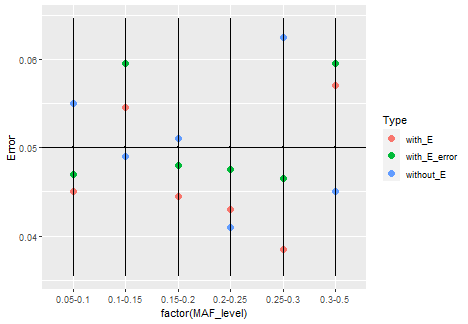
\includegraphics{stats-gene-research-progress-v9_files/figure-latex/unnamed-chunk-5-1.png}

The range in each category is computed using
\(\alpha \pm 3\sqrt{\alpha\times(1-\alpha)/\text{num.rep}}\). Note that
for very low MAF level (0.05-0.1), the type I error rate of our proposed
method seems invalid. However, as MAF level increases, all the methods
seem to have correct type I error behaviors.

\clearpage

\hypertarget{simulation-with-auxiliary-variable}{%
\subsection{Simulation with Auxiliary
Variable:}\label{simulation-with-auxiliary-variable}}

Now, assumes that the true underlying model has the form:
\[Y^* = \beta_0 + \beta_GG_k + \beta_EE+\gamma G_kE +\beta_ZZ + \epsilon\]
where \(Z\) is an auxiliary variable which is known to have no
interaction with environmental variable \(E\).

\hypertarget{analysis-of-1kgp-data-with-one-casual-gene}{%
\subsubsection{Analysis of 1KGP data with one casual
gene:}\label{analysis-of-1kgp-data-with-one-casual-gene}}

Here we repeat the same procedure on the 1kGP data set, assuming that
there is one casual gene in the model

\begin{Shaded}
\begin{Highlighting}[]
\KeywordTok{set.seed}\NormalTok{(}\DecValTok{123}\NormalTok{,}\DataTypeTok{sample.kind=}\StringTok{"Rounding"}\NormalTok{)}
\NormalTok{indx <-}\StringTok{ }\DecValTok{1}\OperatorTok{:}\KeywordTok{ncol}\NormalTok{(G)}

\NormalTok{G_using <-}\StringTok{ }\NormalTok{G[,indx]}
\NormalTok{CHR_using <-}\StringTok{ }\NormalTok{CHR[indx]}
\NormalTok{POS_using <-}\StringTok{ }\NormalTok{POS[indx]}


\CommentTok{### Randomly sample 1 genes:}
\NormalTok{p <-}\StringTok{ }\DecValTok{1}
\CommentTok{### Need to make sure that all genotypes have enough frequencies in the selected genes:}
\NormalTok{freq_counts <-}\StringTok{ }\KeywordTok{big_counts}\NormalTok{(G,}\DataTypeTok{ind.col =}\NormalTok{ indx)}
\NormalTok{MAF <-}\StringTok{ }\KeywordTok{snp_MAF}\NormalTok{(G,}\DataTypeTok{ind.col =}\NormalTok{ indx)}
\NormalTok{Qualified <-}\StringTok{ }\NormalTok{freq_counts[}\DecValTok{3}\NormalTok{,] }\OperatorTok{>=}\StringTok{ }\DecValTok{50} \OperatorTok{&}\StringTok{ }\NormalTok{MAF}\OperatorTok{>=}\FloatTok{0.3}
\NormalTok{POS_EFF <-}\StringTok{ }\KeywordTok{sample}\NormalTok{(POS_using[Qualified], }\DataTypeTok{size =} \DecValTok{1}\NormalTok{)}
\NormalTok{Qualified_}\DecValTok{2}\NormalTok{ <-}\StringTok{ }\NormalTok{freq_counts[}\DecValTok{3}\NormalTok{,] }\OperatorTok{>=}\StringTok{ }\DecValTok{50}
\NormalTok{G_using <-}\StringTok{ }\NormalTok{G[,Qualified_}\DecValTok{2}\NormalTok{]}
\NormalTok{CHR_using <-}\StringTok{ }\NormalTok{CHR[Qualified_}\DecValTok{2}\NormalTok{]}
\NormalTok{POS_using <-}\StringTok{ }\NormalTok{POS[Qualified_}\DecValTok{2}\NormalTok{]}


\CommentTok{### Randomly sample 1/2 genes with strong effects and 1/2 genes with weak effects}
\NormalTok{b0 <-}\StringTok{ }\DecValTok{-1}
\NormalTok{bG <-}\StringTok{ }\FloatTok{0.8}
\NormalTok{bint <-}\StringTok{ }\FloatTok{0.8}
\NormalTok{bE <-}\StringTok{ }\FloatTok{0.1}
\NormalTok{bZ <-}\StringTok{ }\FloatTok{0.3}

\CommentTok{### Generate the underlying environment variable:}
\NormalTok{E <-}\StringTok{ }\KeywordTok{rnorm}\NormalTok{(}\DataTypeTok{n =} \KeywordTok{length}\NormalTok{(G_using[,}\DecValTok{1}\NormalTok{]), }\DataTypeTok{sd =} \DecValTok{1}\NormalTok{)}

\CommentTok{### Generate the auxiliary variable:}
\NormalTok{Z <-}\StringTok{ }\KeywordTok{rnorm}\NormalTok{(}\DataTypeTok{n =} \KeywordTok{length}\NormalTok{(G_using[,}\DecValTok{1}\NormalTok{]), }\DataTypeTok{sd =} \DecValTok{1}\NormalTok{)}

\CommentTok{### Generate the latent variable:}
\NormalTok{y_lat <-}\StringTok{ }\NormalTok{b0 }\OperatorTok{+}\StringTok{ }\NormalTok{bG}\OperatorTok{*}\NormalTok{G_using[,POS_using }\OperatorTok{==}\StringTok{ }\NormalTok{POS_EFF] }\OperatorTok{+}\StringTok{ }\NormalTok{bE}\OperatorTok{*}\NormalTok{E }\OperatorTok{+}\StringTok{ }\NormalTok{bZ}\OperatorTok{*}\NormalTok{Z }\OperatorTok{+}\StringTok{ }\NormalTok{bint}\OperatorTok{*}\NormalTok{E}\OperatorTok{*}\NormalTok{G_using[,POS_using }\OperatorTok{==}\StringTok{ }\NormalTok{POS_EFF] }\OperatorTok{+}\StringTok{ }\KeywordTok{rnorm}\NormalTok{(}\DataTypeTok{n =} \KeywordTok{length}\NormalTok{(G_using[,}\DecValTok{1}\NormalTok{]), }\DataTypeTok{sd =} \FloatTok{0.5}\NormalTok{)}
\NormalTok{case_new <-}\StringTok{ }\KeywordTok{ifelse}\NormalTok{(y_lat }\OperatorTok{>}\StringTok{ }\DecValTok{0}\NormalTok{, }\DecValTok{1}\NormalTok{, }\DecValTok{0}\NormalTok{)}

\CommentTok{### case_control ratio: }
\KeywordTok{table}\NormalTok{(case_new)}
\end{Highlighting}
\end{Shaded}

\begin{verbatim}
## case_new
##    0    1 
## 1175  574
\end{verbatim}

\begin{Shaded}
\begin{Highlighting}[]
\CommentTok{#### Testing for interaction effect}
\CommentTok{### Assuming additive model: Testing for non-linearity}
\NormalTok{waldstats_P1 <-}\StringTok{ }\KeywordTok{c}\NormalTok{()}
\NormalTok{p_vals_P1 <-}\StringTok{ }\KeywordTok{c}\NormalTok{()}

\ControlFlowTok{for}\NormalTok{ (i }\ControlFlowTok{in} \DecValTok{1}\OperatorTok{:}\KeywordTok{ncol}\NormalTok{(G_using)) \{}
\NormalTok{  Gi <-}\StringTok{ }\NormalTok{G_using[,i]}
  
  \ControlFlowTok{if}\NormalTok{(}\KeywordTok{length}\NormalTok{(}\KeywordTok{unique}\NormalTok{(Gi)) }\OperatorTok{!=}\StringTok{ }\DecValTok{3}\NormalTok{)\{}
\NormalTok{    waldstats_P1[i] <-}\StringTok{ }\DecValTok{0}
\NormalTok{    p_vals_P1[i] <-}\StringTok{ }\DecValTok{-1}
\NormalTok{  \}}
  \ControlFlowTok{else}\NormalTok{\{}
\NormalTok{    modi <-}\StringTok{ }\KeywordTok{glm}\NormalTok{(case_new }\OperatorTok{~}\StringTok{ }\KeywordTok{factor}\NormalTok{(Gi)}\OperatorTok{*}\NormalTok{Z, }\DataTypeTok{family =} \KeywordTok{binomial}\NormalTok{(}\DataTypeTok{link =} \StringTok{"probit"}\NormalTok{))}
    \ControlFlowTok{if}\NormalTok{(}\KeywordTok{any}\NormalTok{(}\KeywordTok{is.na}\NormalTok{(modi}\OperatorTok{$}\NormalTok{coefficients)))\{}
\NormalTok{      waldstats_P1[i] <-}\StringTok{ }\DecValTok{0}
\NormalTok{      p_vals_P1[i] <-}\StringTok{ }\DecValTok{-1}
      
\NormalTok{    \}}
    \ControlFlowTok{else}\NormalTok{\{}
\NormalTok{      waldstats_P1[i] <-}\StringTok{ }\KeywordTok{as.numeric}\NormalTok{(aod}\OperatorTok{::}\KeywordTok{wald.test}\NormalTok{(}\KeywordTok{vcov}\NormalTok{(modi)[}\OperatorTok{-}\KeywordTok{c}\NormalTok{(}\DecValTok{1}\NormalTok{,}\DecValTok{4}\NormalTok{),}\OperatorTok{-}\KeywordTok{c}\NormalTok{(}\DecValTok{1}\NormalTok{,}\DecValTok{4}\NormalTok{)], }\DataTypeTok{b =}\NormalTok{ modi}\OperatorTok{$}\NormalTok{coefficients[}\OperatorTok{-}\KeywordTok{c}\NormalTok{(}\DecValTok{1}\NormalTok{,}\DecValTok{4}\NormalTok{)], }\DataTypeTok{H0 =} \KeywordTok{matrix}\NormalTok{(}\DecValTok{0}\NormalTok{,}\DataTypeTok{nrow =} \DecValTok{3}\NormalTok{,}\DataTypeTok{ncol =} \DecValTok{1}\NormalTok{), }\DataTypeTok{L =} \KeywordTok{matrix}\NormalTok{(}\KeywordTok{c}\NormalTok{(}\DecValTok{2}\NormalTok{,}\OperatorTok{-}\DecValTok{1}\NormalTok{,}\DecValTok{0}\NormalTok{,}\DecValTok{0}\NormalTok{,}\DecValTok{0}\NormalTok{,}\DecValTok{0}\NormalTok{,}\DecValTok{1}\NormalTok{,}\DecValTok{0}\NormalTok{,}\DecValTok{0}\NormalTok{,}\DecValTok{0}\NormalTok{,}\DecValTok{0}\NormalTok{,}\DecValTok{1}\NormalTok{),}\DataTypeTok{nrow =} \DecValTok{3}\NormalTok{, }\DataTypeTok{byrow =}\NormalTok{ T))}\OperatorTok{$}\NormalTok{result}\OperatorTok{$}\NormalTok{chi2[}\DecValTok{1}\NormalTok{])}
\NormalTok{      p_vals_P1[i] <-}\StringTok{ }\KeywordTok{as.numeric}\NormalTok{(aod}\OperatorTok{::}\KeywordTok{wald.test}\NormalTok{(}\KeywordTok{vcov}\NormalTok{(modi)[}\OperatorTok{-}\KeywordTok{c}\NormalTok{(}\DecValTok{1}\NormalTok{,}\DecValTok{4}\NormalTok{),}\OperatorTok{-}\KeywordTok{c}\NormalTok{(}\DecValTok{1}\NormalTok{,}\DecValTok{4}\NormalTok{)], }\DataTypeTok{b =}\NormalTok{ modi}\OperatorTok{$}\NormalTok{coefficients[}\OperatorTok{-}\KeywordTok{c}\NormalTok{(}\DecValTok{1}\NormalTok{,}\DecValTok{4}\NormalTok{)], }\DataTypeTok{H0 =} \KeywordTok{matrix}\NormalTok{(}\DecValTok{0}\NormalTok{,}\DataTypeTok{nrow =} \DecValTok{3}\NormalTok{,}\DataTypeTok{ncol =} \DecValTok{1}\NormalTok{), }\DataTypeTok{L =} \KeywordTok{matrix}\NormalTok{(}\KeywordTok{c}\NormalTok{(}\DecValTok{2}\NormalTok{,}\OperatorTok{-}\DecValTok{1}\NormalTok{,}\DecValTok{0}\NormalTok{,}\DecValTok{0}\NormalTok{,}\DecValTok{0}\NormalTok{,}\DecValTok{0}\NormalTok{,}\DecValTok{1}\NormalTok{,}\DecValTok{0}\NormalTok{,}\DecValTok{0}\NormalTok{,}\DecValTok{0}\NormalTok{,}\DecValTok{0}\NormalTok{,}\DecValTok{1}\NormalTok{),}\DataTypeTok{nrow =} \DecValTok{3}\NormalTok{, }\DataTypeTok{byrow =}\NormalTok{ T))}\OperatorTok{$}\NormalTok{result}\OperatorTok{$}\NormalTok{chi2[}\DecValTok{3}\NormalTok{]) }
\NormalTok{    \}}
\NormalTok{  \}}
\NormalTok{\}}

\NormalTok{result_P_INT <-}\StringTok{ }\KeywordTok{tibble}\NormalTok{(}\DataTypeTok{SNP =}\NormalTok{ obj.bigSNP}\OperatorTok{$}\NormalTok{map}\OperatorTok{$}\NormalTok{marker.ID[Qualified_}\DecValTok{2}\NormalTok{], }\DataTypeTok{CHR =}\NormalTok{ CHR_using, }\DataTypeTok{BP =}\NormalTok{ POS_using , }\DataTypeTok{stats =}\NormalTok{ waldstats_P1, }\DataTypeTok{P =}\NormalTok{ p_vals_P1) }\OperatorTok\StringTok{ }\KeywordTok{filter}\NormalTok{(P }\OperatorTok{>}\StringTok{ }\DecValTok{0}\NormalTok{)}
\KeywordTok{manhattan}\NormalTok{(result_P_INT, }\DataTypeTok{highlight =}\NormalTok{ result_P_INT}\OperatorTok{$}\NormalTok{SNP[}\KeywordTok{which}\NormalTok{(POS_using }\OperatorTok\StringTok{ }\NormalTok{POS_EFF)], }\DataTypeTok{suggestiveline =} \OtherTok{FALSE}\NormalTok{, }\DataTypeTok{genomewideline =} \OperatorTok{-}\KeywordTok{log10}\NormalTok{(}\DecValTok{5} \OperatorTok{*}\StringTok{ }\NormalTok{(}\DecValTok{10} \OperatorTok{^}\StringTok{ }\DecValTok{-8}\NormalTok{)))}
\end{Highlighting}
\end{Shaded}

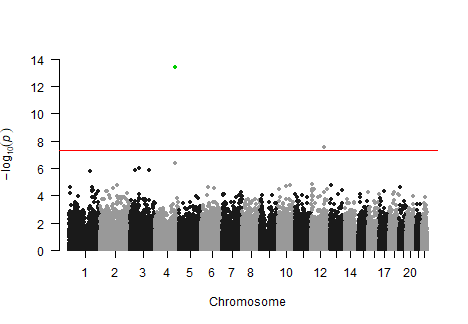
\includegraphics{stats-gene-research-progress-v9_files/figure-latex/unnamed-chunk-7-1.png}

\begin{Shaded}
\begin{Highlighting}[]
\KeywordTok{qq}\NormalTok{(}\KeywordTok{na.omit}\NormalTok{(result_P_INT)}\OperatorTok{$}\NormalTok{P)}
\end{Highlighting}
\end{Shaded}

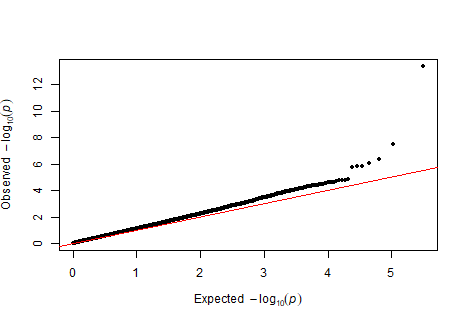
\includegraphics{stats-gene-research-progress-v9_files/figure-latex/unnamed-chunk-7-2.png}

\begin{Shaded}
\begin{Highlighting}[]
\KeywordTok{hist}\NormalTok{(result_P_INT}\OperatorTok{$}\NormalTok{P, }\DataTypeTok{breaks =} \DecValTok{30}\NormalTok{)}
\end{Highlighting}
\end{Shaded}

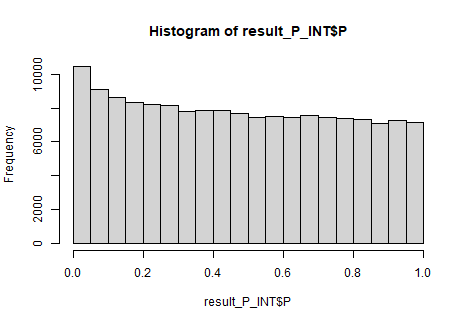
\includegraphics{stats-gene-research-progress-v9_files/figure-latex/unnamed-chunk-7-3.png}

\clearpage

\hypertarget{power-comparison-1}{%
\subsubsection{Power Comparison:}\label{power-comparison-1}}

Here we consider the following parameter specification:

\begin{itemize}
\tightlist
\item
  \(\beta_0= -1, \beta_G=0.8, \beta_E= 0.2,\gamma=0.4, \beta_Z=0.8\)
\item
  \(E \sim N(0,1)\)
\item
  \(\epsilon \sim N(0,0.5)\) The \(G_k\) will be sampled for six times,
  with different levels of MAF in each time.
\end{itemize}

\begin{Shaded}
\begin{Highlighting}[]
\KeywordTok{set.seed}\NormalTok{(}\DecValTok{123}\NormalTok{,}\DataTypeTok{sample.kind=}\StringTok{"Rounding"}\NormalTok{)}
\NormalTok{indx <-}\StringTok{ }\DecValTok{1}\OperatorTok{:}\KeywordTok{ncol}\NormalTok{(G)}

\NormalTok{G_using <-}\StringTok{ }\NormalTok{G[,indx]}
\NormalTok{CHR_using <-}\StringTok{ }\NormalTok{CHR[indx]}
\NormalTok{POS_using <-}\StringTok{ }\NormalTok{POS[indx]}

\CommentTok{### Sample three casual genes, corresponding to different MAF}
\NormalTok{freq_counts <-}\StringTok{ }\KeywordTok{big_counts}\NormalTok{(G,}\DataTypeTok{ind.col =}\NormalTok{ indx)}
\NormalTok{MAF <-}\StringTok{ }\KeywordTok{snp_MAF}\NormalTok{(G,}\DataTypeTok{ind.col =}\NormalTok{ indx)}
\NormalTok{Qualified <-}\StringTok{ }\NormalTok{freq_counts[}\DecValTok{3}\NormalTok{,] }\OperatorTok{>=}\StringTok{ }\DecValTok{30} \OperatorTok{&}\StringTok{ }\NormalTok{MAF}\OperatorTok{>=}\FloatTok{0.05} \OperatorTok{&}\StringTok{ }\NormalTok{MAF}\OperatorTok{<=}\FloatTok{0.1}
\NormalTok{POS_EFF1 <-}\StringTok{ }\KeywordTok{sample}\NormalTok{(POS_using[Qualified], }\DataTypeTok{size =} \DecValTok{1}\NormalTok{)}
\NormalTok{Qualified <-}\StringTok{ }\NormalTok{freq_counts[}\DecValTok{3}\NormalTok{,] }\OperatorTok{>=}\StringTok{ }\DecValTok{50} \OperatorTok{&}\StringTok{ }\NormalTok{MAF}\OperatorTok{>=}\FloatTok{0.1} \OperatorTok{&}\StringTok{ }\NormalTok{MAF}\OperatorTok{<=}\FloatTok{0.15}
\NormalTok{POS_EFF2 <-}\StringTok{ }\KeywordTok{sample}\NormalTok{(POS_using[Qualified], }\DataTypeTok{size =} \DecValTok{1}\NormalTok{)}
\NormalTok{Qualified <-}\StringTok{ }\NormalTok{freq_counts[}\DecValTok{3}\NormalTok{,] }\OperatorTok{>=}\StringTok{ }\DecValTok{80} \OperatorTok{&}\StringTok{ }\NormalTok{MAF}\OperatorTok{>=}\FloatTok{0.15} \OperatorTok{&}\StringTok{ }\NormalTok{MAF}\OperatorTok{<=}\FloatTok{0.2}
\NormalTok{POS_EFF3 <-}\StringTok{ }\KeywordTok{sample}\NormalTok{(POS_using[Qualified], }\DataTypeTok{size =} \DecValTok{1}\NormalTok{)}
\NormalTok{Qualified <-}\StringTok{ }\NormalTok{freq_counts[}\DecValTok{3}\NormalTok{,] }\OperatorTok{>=}\StringTok{ }\DecValTok{80} \OperatorTok{&}\StringTok{ }\NormalTok{MAF}\OperatorTok{>=}\FloatTok{0.2} \OperatorTok{&}\StringTok{ }\NormalTok{MAF}\OperatorTok{<=}\FloatTok{0.3}
\NormalTok{POS_EFF4 <-}\StringTok{ }\KeywordTok{sample}\NormalTok{(POS_using[Qualified], }\DataTypeTok{size =} \DecValTok{1}\NormalTok{)}
\NormalTok{Qualified <-}\StringTok{ }\NormalTok{freq_counts[}\DecValTok{3}\NormalTok{,] }\OperatorTok{>=}\StringTok{ }\DecValTok{100} \OperatorTok{&}\StringTok{ }\NormalTok{MAF}\OperatorTok{>=}\FloatTok{0.3} \OperatorTok{&}\StringTok{ }\NormalTok{MAF}\OperatorTok{<=}\FloatTok{0.4}
\NormalTok{POS_EFF5 <-}\StringTok{ }\KeywordTok{sample}\NormalTok{(POS_using[Qualified], }\DataTypeTok{size =} \DecValTok{1}\NormalTok{)}
\NormalTok{Qualified <-}\StringTok{ }\NormalTok{freq_counts[}\DecValTok{3}\NormalTok{,] }\OperatorTok{>=}\StringTok{ }\DecValTok{100} \OperatorTok{&}\StringTok{ }\NormalTok{MAF}\OperatorTok{>=}\FloatTok{0.4}
\NormalTok{POS_EFF6 <-}\StringTok{ }\KeywordTok{sample}\NormalTok{(POS_using[Qualified], }\DataTypeTok{size =} \DecValTok{1}\NormalTok{)}


\CommentTok{### Computation:}
\CommentTok{### Compute power of each case:}
\KeywordTok{suppressWarnings}\NormalTok{(power1 <-}\StringTok{ }\KeywordTok{Compare_Aggreg_power_auxiliary}\NormalTok{(}\DataTypeTok{k =} \DecValTok{200}\NormalTok{, }\DataTypeTok{G_using =}\NormalTok{ G_using, }\DataTypeTok{POS_using =}\NormalTok{ POS_using, }\DataTypeTok{effective_gene =}\NormalTok{ POS_EFF1, }\DataTypeTok{sigma_eps =} \FloatTok{0.5}\NormalTok{, }\DataTypeTok{sigmaE =} \DecValTok{1}\NormalTok{))}
\NormalTok{power1 <-}\StringTok{ }\NormalTok{power1 }\OperatorTok{<=}\StringTok{ }\DecValTok{5} \OperatorTok{*}\StringTok{ }\NormalTok{(}\DecValTok{10} \OperatorTok{^}\StringTok{ }\DecValTok{-8}\NormalTok{)}
\NormalTok{power1 <-}\StringTok{ }\KeywordTok{apply}\NormalTok{(power1, }\DataTypeTok{MARGIN =} \DecValTok{2}\NormalTok{, }\DataTypeTok{FUN =}\NormalTok{ mean)}

\KeywordTok{suppressWarnings}\NormalTok{(power2 <-}\StringTok{ }\KeywordTok{Compare_Aggreg_power_auxiliary}\NormalTok{(}\DataTypeTok{k =} \DecValTok{200}\NormalTok{, }\DataTypeTok{G_using =}\NormalTok{ G_using, }\DataTypeTok{POS_using =}\NormalTok{ POS_using, }\DataTypeTok{effective_gene =}\NormalTok{ POS_EFF2, }\DataTypeTok{sigma_eps =} \FloatTok{0.5}\NormalTok{, }\DataTypeTok{sigmaE =} \DecValTok{1}\NormalTok{))}
\NormalTok{power2 <-}\StringTok{ }\NormalTok{power2 }\OperatorTok{<=}\StringTok{ }\DecValTok{5} \OperatorTok{*}\StringTok{ }\NormalTok{(}\DecValTok{10} \OperatorTok{^}\StringTok{ }\DecValTok{-8}\NormalTok{)}
\NormalTok{power2 <-}\StringTok{ }\KeywordTok{apply}\NormalTok{(power2, }\DataTypeTok{MARGIN =} \DecValTok{2}\NormalTok{, }\DataTypeTok{FUN =}\NormalTok{ mean)}

\KeywordTok{suppressWarnings}\NormalTok{(power3 <-}\StringTok{ }\KeywordTok{Compare_Aggreg_power_auxiliary}\NormalTok{(}\DataTypeTok{k =} \DecValTok{200}\NormalTok{, }\DataTypeTok{G_using =}\NormalTok{ G_using, }\DataTypeTok{POS_using =}\NormalTok{ POS_using, }\DataTypeTok{effective_gene =}\NormalTok{ POS_EFF3, }\DataTypeTok{sigma_eps =} \FloatTok{0.5}\NormalTok{, }\DataTypeTok{sigmaE =} \DecValTok{1}\NormalTok{))}
\NormalTok{power3 <-}\StringTok{ }\NormalTok{power3 }\OperatorTok{<=}\StringTok{ }\DecValTok{5} \OperatorTok{*}\StringTok{ }\NormalTok{(}\DecValTok{10} \OperatorTok{^}\StringTok{ }\DecValTok{-8}\NormalTok{)}
\NormalTok{power3 <-}\StringTok{ }\KeywordTok{apply}\NormalTok{(power3, }\DataTypeTok{MARGIN =} \DecValTok{2}\NormalTok{, }\DataTypeTok{FUN =}\NormalTok{ mean)}

\KeywordTok{suppressWarnings}\NormalTok{(power4 <-}\StringTok{ }\KeywordTok{Compare_Aggreg_power_auxiliary}\NormalTok{(}\DataTypeTok{k =} \DecValTok{200}\NormalTok{, }\DataTypeTok{G_using =}\NormalTok{ G_using, }\DataTypeTok{POS_using =}\NormalTok{ POS_using, }\DataTypeTok{effective_gene =}\NormalTok{ POS_EFF4, }\DataTypeTok{sigma_eps =} \FloatTok{0.5}\NormalTok{, }\DataTypeTok{sigmaE =} \DecValTok{1}\NormalTok{))}
\NormalTok{power4 <-}\StringTok{ }\NormalTok{power4 }\OperatorTok{<=}\StringTok{ }\DecValTok{5} \OperatorTok{*}\StringTok{ }\NormalTok{(}\DecValTok{10} \OperatorTok{^}\StringTok{ }\DecValTok{-8}\NormalTok{)}
\NormalTok{power4 <-}\StringTok{ }\KeywordTok{apply}\NormalTok{(power4, }\DataTypeTok{MARGIN =} \DecValTok{2}\NormalTok{, }\DataTypeTok{FUN =}\NormalTok{ mean)}

\KeywordTok{suppressWarnings}\NormalTok{(power5 <-}\StringTok{ }\KeywordTok{Compare_Aggreg_power_auxiliary}\NormalTok{(}\DataTypeTok{k =} \DecValTok{200}\NormalTok{, }\DataTypeTok{G_using =}\NormalTok{ G_using, }\DataTypeTok{POS_using =}\NormalTok{ POS_using, }\DataTypeTok{effective_gene =}\NormalTok{ POS_EFF5, }\DataTypeTok{sigma_eps =} \FloatTok{0.5}\NormalTok{, }\DataTypeTok{sigmaE =} \DecValTok{1}\NormalTok{))}
\NormalTok{power5 <-}\StringTok{ }\NormalTok{power5 }\OperatorTok{<=}\StringTok{ }\DecValTok{5} \OperatorTok{*}\StringTok{ }\NormalTok{(}\DecValTok{10} \OperatorTok{^}\StringTok{ }\DecValTok{-8}\NormalTok{)}
\NormalTok{power5 <-}\StringTok{ }\KeywordTok{apply}\NormalTok{(power5, }\DataTypeTok{MARGIN =} \DecValTok{2}\NormalTok{, }\DataTypeTok{FUN =}\NormalTok{ mean)}

\KeywordTok{suppressWarnings}\NormalTok{(power6 <-}\StringTok{ }\KeywordTok{Compare_Aggreg_power_auxiliary}\NormalTok{(}\DataTypeTok{k =} \DecValTok{200}\NormalTok{, }\DataTypeTok{G_using =}\NormalTok{ G_using, }\DataTypeTok{POS_using =}\NormalTok{ POS_using, }\DataTypeTok{effective_gene =}\NormalTok{ POS_EFF6, }\DataTypeTok{sigma_eps =} \FloatTok{0.5}\NormalTok{, }\DataTypeTok{sigmaE =} \DecValTok{1}\NormalTok{))}
\NormalTok{power6 <-}\StringTok{ }\NormalTok{power6 }\OperatorTok{<=}\StringTok{ }\DecValTok{5} \OperatorTok{*}\StringTok{ }\NormalTok{(}\DecValTok{10} \OperatorTok{^}\StringTok{ }\DecValTok{-8}\NormalTok{)}
\NormalTok{power6 <-}\StringTok{ }\KeywordTok{apply}\NormalTok{(power6, }\DataTypeTok{MARGIN =} \DecValTok{2}\NormalTok{, }\DataTypeTok{FUN =}\NormalTok{ mean)}

\CommentTok{## Table:}
\NormalTok{power <-}\StringTok{ }\KeywordTok{as_tibble}\NormalTok{(}\KeywordTok{as.matrix}\NormalTok{(}\KeywordTok{rbind}\NormalTok{(power1,power2,power3, power4,power5,power6))) }\OperatorTok\StringTok{ }\KeywordTok{mutate}\NormalTok{(}\DataTypeTok{MAF =} \KeywordTok{sort}\NormalTok{(MAF[POS_using }\OperatorTok\StringTok{ }\KeywordTok{c}\NormalTok{(POS_EFF1,POS_EFF2,POS_EFF3,POS_EFF4,POS_EFF5,POS_EFF6)]))}
\NormalTok{kableExtra}\OperatorTok{::}\KeywordTok{kable}\NormalTok{(power,}\DataTypeTok{caption =} \StringTok{"Comparison of Power"}\NormalTok{)}
\end{Highlighting}
\end{Shaded}

\begin{table}

\caption{\label{tab:unnamed-chunk-8}Comparison of Power}
\centering
\begin{tabular}[t]{r|r|r|r|r}
\hline
proposed\_1 & proposed\_2 & oracle & oracle\_error & MAF\\
\hline
0.005 & 0.070 & 0.680 & 0.310 & 0.0737564\\
\hline
0.020 & 0.110 & 0.980 & 0.855 & 0.1463694\\
\hline
0.055 & 0.205 & 0.995 & 0.960 & 0.1803888\\
\hline
0.050 & 0.170 & 1.000 & 1.000 & 0.2172670\\
\hline
0.070 & 0.250 & 1.000 & 1.000 & 0.3070326\\
\hline
0.040 & 0.175 & 1.000 & 1.000 & 0.4568325\\
\hline
\end{tabular}
\end{table}

\begin{Shaded}
\begin{Highlighting}[]
\CommentTok{## Figure:}

\NormalTok{power_plot <-}\StringTok{ }\NormalTok{power }\OperatorTok\StringTok{ }\KeywordTok{pivot_longer}\NormalTok{(proposed_}\DecValTok{1}\OperatorTok{:}\NormalTok{oracle_error, }\StringTok{"Type"}\NormalTok{, }\DataTypeTok{values_to =} \StringTok{"Power"}\NormalTok{) }\OperatorTok\StringTok{ }\KeywordTok{mutate}\NormalTok{(}\DataTypeTok{Type =} \KeywordTok{factor}\NormalTok{(Type))}
\KeywordTok{levels}\NormalTok{(power_plot}\OperatorTok{$}\NormalTok{Type) <-}\StringTok{ }\KeywordTok{c}\NormalTok{(}\StringTok{"with_E"}\NormalTok{,}\StringTok{"with_E_error"}\NormalTok{, }\StringTok{"without_E_1df"}\NormalTok{, }\StringTok{"without_E_3df"}\NormalTok{)}
\NormalTok{power_plot }\OperatorTok\StringTok{ }\KeywordTok{ggplot}\NormalTok{(}\KeywordTok{aes}\NormalTok{(MAF,Power,}\DataTypeTok{color =}\NormalTok{ Type)) }\OperatorTok{+}\StringTok{ }\KeywordTok{geom_line}\NormalTok{()}
\end{Highlighting}
\end{Shaded}

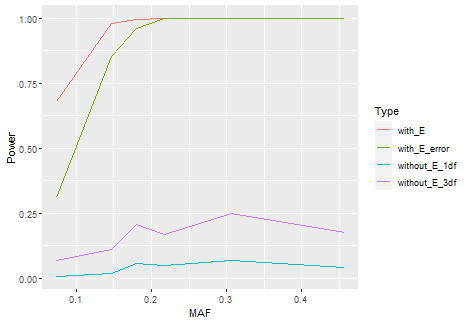
\includegraphics{stats-gene-research-progress-v9_files/figure-latex/unnamed-chunk-8-1.png}

In this parameter setting, we can see that even though with the help
from the auxiliary variable \texttt{z}, the power is increased
significantly. The proposed methods still in generally have much lower
power than the oracle method using information of \texttt{E}, regardless
whether there is measurement error in \texttt{E}.

Next, we will make a more optimistic parameter setting, by increasing
\(\gamma\) from \(0.4\) to \(0.8\), and do the power comparison again:

\begin{Shaded}
\begin{Highlighting}[]
\KeywordTok{set.seed}\NormalTok{(}\DecValTok{123}\NormalTok{,}\DataTypeTok{sample.kind=}\StringTok{"Rounding"}\NormalTok{)}

\CommentTok{### Computation:}
\CommentTok{### Compute power of each case:}
\KeywordTok{suppressWarnings}\NormalTok{(power1 <-}\StringTok{ }\KeywordTok{Compare_Aggreg_power_auxiliary}\NormalTok{(}\DataTypeTok{k =} \DecValTok{200}\NormalTok{, }\DataTypeTok{G_using =}\NormalTok{ G_using, }\DataTypeTok{POS_using =}\NormalTok{ POS_using, }\DataTypeTok{effective_gene =}\NormalTok{ POS_EFF1, }\DataTypeTok{sigma_eps =} \FloatTok{0.5}\NormalTok{, }\DataTypeTok{sigmaE =} \DecValTok{1}\NormalTok{, }\DataTypeTok{bint1 =} \FloatTok{0.8}\NormalTok{))}
\NormalTok{power1 <-}\StringTok{ }\NormalTok{power1 }\OperatorTok{<=}\StringTok{ }\DecValTok{5} \OperatorTok{*}\StringTok{ }\NormalTok{(}\DecValTok{10} \OperatorTok{^}\StringTok{ }\DecValTok{-8}\NormalTok{)}
\NormalTok{power1 <-}\StringTok{ }\KeywordTok{apply}\NormalTok{(power1, }\DataTypeTok{MARGIN =} \DecValTok{2}\NormalTok{, }\DataTypeTok{FUN =}\NormalTok{ mean)}

\KeywordTok{suppressWarnings}\NormalTok{(power2 <-}\StringTok{ }\KeywordTok{Compare_Aggreg_power_auxiliary}\NormalTok{(}\DataTypeTok{k =} \DecValTok{200}\NormalTok{, }\DataTypeTok{G_using =}\NormalTok{ G_using, }\DataTypeTok{POS_using =}\NormalTok{ POS_using, }\DataTypeTok{effective_gene =}\NormalTok{ POS_EFF2, }\DataTypeTok{sigma_eps =} \FloatTok{0.5}\NormalTok{, }\DataTypeTok{sigmaE =} \DecValTok{1}\NormalTok{, }\DataTypeTok{bint1 =} \FloatTok{0.8}\NormalTok{))}
\NormalTok{power2 <-}\StringTok{ }\NormalTok{power2 }\OperatorTok{<=}\StringTok{ }\DecValTok{5} \OperatorTok{*}\StringTok{ }\NormalTok{(}\DecValTok{10} \OperatorTok{^}\StringTok{ }\DecValTok{-8}\NormalTok{)}
\NormalTok{power2 <-}\StringTok{ }\KeywordTok{apply}\NormalTok{(power2, }\DataTypeTok{MARGIN =} \DecValTok{2}\NormalTok{, }\DataTypeTok{FUN =}\NormalTok{ mean)}

\KeywordTok{suppressWarnings}\NormalTok{(power3 <-}\StringTok{ }\KeywordTok{Compare_Aggreg_power_auxiliary}\NormalTok{(}\DataTypeTok{k =} \DecValTok{200}\NormalTok{, }\DataTypeTok{G_using =}\NormalTok{ G_using, }\DataTypeTok{POS_using =}\NormalTok{ POS_using, }\DataTypeTok{effective_gene =}\NormalTok{ POS_EFF3, }\DataTypeTok{sigma_eps =} \FloatTok{0.5}\NormalTok{, }\DataTypeTok{sigmaE =} \DecValTok{1}\NormalTok{, }\DataTypeTok{bint1 =} \FloatTok{0.8}\NormalTok{))}
\NormalTok{power3 <-}\StringTok{ }\NormalTok{power3 }\OperatorTok{<=}\StringTok{ }\DecValTok{5} \OperatorTok{*}\StringTok{ }\NormalTok{(}\DecValTok{10} \OperatorTok{^}\StringTok{ }\DecValTok{-8}\NormalTok{)}
\NormalTok{power3 <-}\StringTok{ }\KeywordTok{apply}\NormalTok{(power3, }\DataTypeTok{MARGIN =} \DecValTok{2}\NormalTok{, }\DataTypeTok{FUN =}\NormalTok{ mean)}

\KeywordTok{suppressWarnings}\NormalTok{(power4 <-}\StringTok{ }\KeywordTok{Compare_Aggreg_power_auxiliary}\NormalTok{(}\DataTypeTok{k =} \DecValTok{200}\NormalTok{, }\DataTypeTok{G_using =}\NormalTok{ G_using, }\DataTypeTok{POS_using =}\NormalTok{ POS_using, }\DataTypeTok{effective_gene =}\NormalTok{ POS_EFF4, }\DataTypeTok{sigma_eps =} \FloatTok{0.5}\NormalTok{, }\DataTypeTok{sigmaE =} \DecValTok{1}\NormalTok{, }\DataTypeTok{bint1 =} \FloatTok{0.8}\NormalTok{))}
\NormalTok{power4 <-}\StringTok{ }\NormalTok{power4 }\OperatorTok{<=}\StringTok{ }\DecValTok{5} \OperatorTok{*}\StringTok{ }\NormalTok{(}\DecValTok{10} \OperatorTok{^}\StringTok{ }\DecValTok{-8}\NormalTok{)}
\NormalTok{power4 <-}\StringTok{ }\KeywordTok{apply}\NormalTok{(power4, }\DataTypeTok{MARGIN =} \DecValTok{2}\NormalTok{, }\DataTypeTok{FUN =}\NormalTok{ mean)}

\KeywordTok{suppressWarnings}\NormalTok{(power5 <-}\StringTok{ }\KeywordTok{Compare_Aggreg_power_auxiliary}\NormalTok{(}\DataTypeTok{k =} \DecValTok{200}\NormalTok{, }\DataTypeTok{G_using =}\NormalTok{ G_using, }\DataTypeTok{POS_using =}\NormalTok{ POS_using, }\DataTypeTok{effective_gene =}\NormalTok{ POS_EFF5, }\DataTypeTok{sigma_eps =} \FloatTok{0.5}\NormalTok{, }\DataTypeTok{sigmaE =} \DecValTok{1}\NormalTok{, }\DataTypeTok{bint1 =} \FloatTok{0.8}\NormalTok{))}
\NormalTok{power5 <-}\StringTok{ }\NormalTok{power5 }\OperatorTok{<=}\StringTok{ }\DecValTok{5} \OperatorTok{*}\StringTok{ }\NormalTok{(}\DecValTok{10} \OperatorTok{^}\StringTok{ }\DecValTok{-8}\NormalTok{)}
\NormalTok{power5 <-}\StringTok{ }\KeywordTok{apply}\NormalTok{(power5, }\DataTypeTok{MARGIN =} \DecValTok{2}\NormalTok{, }\DataTypeTok{FUN =}\NormalTok{ mean)}

\KeywordTok{suppressWarnings}\NormalTok{(power6 <-}\StringTok{ }\KeywordTok{Compare_Aggreg_power_auxiliary}\NormalTok{(}\DataTypeTok{k =} \DecValTok{200}\NormalTok{, }\DataTypeTok{G_using =}\NormalTok{ G_using, }\DataTypeTok{POS_using =}\NormalTok{ POS_using, }\DataTypeTok{effective_gene =}\NormalTok{ POS_EFF6, }\DataTypeTok{sigma_eps =} \FloatTok{0.5}\NormalTok{, }\DataTypeTok{sigmaE =} \DecValTok{1}\NormalTok{, }\DataTypeTok{bint1 =} \FloatTok{0.8}\NormalTok{))}
\NormalTok{power6 <-}\StringTok{ }\NormalTok{power6 }\OperatorTok{<=}\StringTok{ }\DecValTok{5} \OperatorTok{*}\StringTok{ }\NormalTok{(}\DecValTok{10} \OperatorTok{^}\StringTok{ }\DecValTok{-8}\NormalTok{)}
\NormalTok{power6 <-}\StringTok{ }\KeywordTok{apply}\NormalTok{(power6, }\DataTypeTok{MARGIN =} \DecValTok{2}\NormalTok{, }\DataTypeTok{FUN =}\NormalTok{ mean)}
\CommentTok{## Table:}
\NormalTok{power <-}\StringTok{ }\KeywordTok{as_tibble}\NormalTok{(}\KeywordTok{as.matrix}\NormalTok{(}\KeywordTok{rbind}\NormalTok{(power1,power2,power3, power4,power5,power6))) }\OperatorTok\StringTok{ }\KeywordTok{mutate}\NormalTok{(}\DataTypeTok{MAF =} \KeywordTok{sort}\NormalTok{(MAF[POS_using }\OperatorTok\StringTok{ }\KeywordTok{c}\NormalTok{(POS_EFF1,POS_EFF2,POS_EFF3,POS_EFF4,POS_EFF5,POS_EFF6)]))}
\NormalTok{kableExtra}\OperatorTok{::}\KeywordTok{kable}\NormalTok{(power,}\DataTypeTok{caption =} \StringTok{"Comparison of Power"}\NormalTok{)}
\end{Highlighting}
\end{Shaded}

\begin{table}

\caption{\label{tab:unnamed-chunk-9}Comparison of Power}
\centering
\begin{tabular}[t]{r|r|r|r|r}
\hline
proposed\_1 & proposed\_2 & oracle & oracle\_error & MAF\\
\hline
0.050 & 0.740 & 1 & 0.985 & 0.0737564\\
\hline
0.300 & 0.925 & 1 & 1.000 & 0.1463694\\
\hline
0.535 & 0.990 & 1 & 1.000 & 0.1803888\\
\hline
0.640 & 0.975 & 1 & 1.000 & 0.2172670\\
\hline
0.865 & 0.985 & 1 & 1.000 & 0.3070326\\
\hline
0.830 & 0.985 & 1 & 1.000 & 0.4568325\\
\hline
\end{tabular}
\end{table}

\begin{Shaded}
\begin{Highlighting}[]
\CommentTok{## Figure:}
\NormalTok{power_plot <-}\StringTok{ }\NormalTok{power }\OperatorTok\StringTok{ }\KeywordTok{pivot_longer}\NormalTok{(proposed_}\DecValTok{1}\OperatorTok{:}\NormalTok{oracle_error, }\StringTok{"Type"}\NormalTok{, }\DataTypeTok{values_to =} \StringTok{"Power"}\NormalTok{) }\OperatorTok\StringTok{ }\KeywordTok{mutate}\NormalTok{(}\DataTypeTok{Type =} \KeywordTok{factor}\NormalTok{(Type))}
\KeywordTok{levels}\NormalTok{(power_plot}\OperatorTok{$}\NormalTok{Type) <-}\StringTok{ }\KeywordTok{c}\NormalTok{(}\StringTok{"with_E"}\NormalTok{,}\StringTok{"with_E_error"}\NormalTok{, }\StringTok{"without_E_1df"}\NormalTok{, }\StringTok{"without_E_3df"}\NormalTok{)}
\NormalTok{power_plot }\OperatorTok\StringTok{ }\KeywordTok{ggplot}\NormalTok{(}\KeywordTok{aes}\NormalTok{(MAF,Power,}\DataTypeTok{color =}\NormalTok{ Type)) }\OperatorTok{+}\StringTok{ }\KeywordTok{geom_line}\NormalTok{()}
\end{Highlighting}
\end{Shaded}

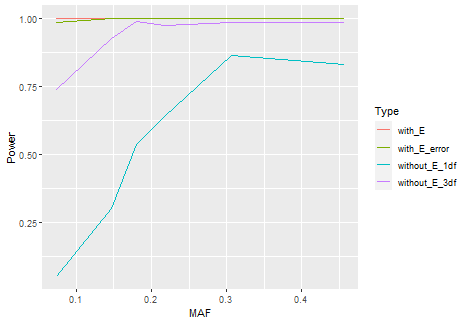
\includegraphics{stats-gene-research-progress-v9_files/figure-latex/unnamed-chunk-9-1.png}

From the plot above, we can notice that the difference becomes smaller
as \(\gamma\) gets larger.

\clearpage

\hypertarget{type-i-error-comparison-1}{%
\subsubsection{Type I error
Comparison:}\label{type-i-error-comparison-1}}

Still consider the setting:

\begin{itemize}
\tightlist
\item
  \(\beta_0= -1, \beta_G=0.8, \beta_E= 0.2,\gamma=0.8, \beta_Z=0.8\)
\item
  \(E \sim N(0,1)\)
\item
  \(\epsilon \sim N(0,0.5)\) Now, we aim to compare the type I error
  rate of these procedures at different MAF levels:
\end{itemize}

\begin{Shaded}
\begin{Highlighting}[]
\KeywordTok{set.seed}\NormalTok{(}\DecValTok{123}\NormalTok{,}\DataTypeTok{sample.kind=}\StringTok{"Rounding"}\NormalTok{)}

\CommentTok{### Sample three casual genes, corresponding to different MAF}
\CommentTok{### Sample three casual genes, corresponding to different MAF}
\NormalTok{freq_counts <-}\StringTok{ }\KeywordTok{big_counts}\NormalTok{(G,}\DataTypeTok{ind.col =}\NormalTok{ indx)}
\NormalTok{MAF <-}\StringTok{ }\KeywordTok{snp_MAF}\NormalTok{(G,}\DataTypeTok{ind.col =}\NormalTok{ indx)}
\NormalTok{Qualified <-}\StringTok{ }\NormalTok{freq_counts[}\DecValTok{3}\NormalTok{,] }\OperatorTok{>=}\StringTok{ }\DecValTok{30} \OperatorTok{&}\StringTok{ }\NormalTok{MAF}\OperatorTok{>=}\FloatTok{0.05} \OperatorTok{&}\StringTok{ }\NormalTok{MAF}\OperatorTok{<=}\FloatTok{0.1}
\NormalTok{POS_EFF1 <-}\StringTok{ }\KeywordTok{sample}\NormalTok{(POS_using[Qualified], }\DataTypeTok{size =} \DecValTok{1}\NormalTok{)}
\NormalTok{Qualified <-}\StringTok{ }\NormalTok{freq_counts[}\DecValTok{3}\NormalTok{,] }\OperatorTok{>=}\StringTok{ }\DecValTok{50} \OperatorTok{&}\StringTok{ }\NormalTok{MAF}\OperatorTok{>=}\FloatTok{0.1} \OperatorTok{&}\StringTok{ }\NormalTok{MAF}\OperatorTok{<=}\FloatTok{0.15}
\NormalTok{POS_EFF2 <-}\StringTok{ }\KeywordTok{sample}\NormalTok{(POS_using[Qualified], }\DataTypeTok{size =} \DecValTok{1}\NormalTok{)}
\NormalTok{Qualified <-}\StringTok{ }\NormalTok{freq_counts[}\DecValTok{3}\NormalTok{,] }\OperatorTok{>=}\StringTok{ }\DecValTok{80} \OperatorTok{&}\StringTok{ }\NormalTok{MAF}\OperatorTok{>=}\FloatTok{0.15} \OperatorTok{&}\StringTok{ }\NormalTok{MAF}\OperatorTok{<=}\FloatTok{0.2}
\NormalTok{POS_EFF3 <-}\StringTok{ }\KeywordTok{sample}\NormalTok{(POS_using[Qualified], }\DataTypeTok{size =} \DecValTok{1}\NormalTok{)}
\NormalTok{Qualified <-}\StringTok{ }\NormalTok{freq_counts[}\DecValTok{3}\NormalTok{,] }\OperatorTok{>=}\StringTok{ }\DecValTok{80} \OperatorTok{&}\StringTok{ }\NormalTok{MAF}\OperatorTok{>=}\FloatTok{0.2} \OperatorTok{&}\StringTok{ }\NormalTok{MAF}\OperatorTok{<=}\FloatTok{0.25}
\NormalTok{POS_EFF4 <-}\StringTok{ }\KeywordTok{sample}\NormalTok{(POS_using[Qualified], }\DataTypeTok{size =} \DecValTok{1}\NormalTok{)}
\NormalTok{Qualified <-}\StringTok{ }\NormalTok{freq_counts[}\DecValTok{3}\NormalTok{,] }\OperatorTok{>=}\StringTok{ }\DecValTok{100} \OperatorTok{&}\StringTok{ }\NormalTok{MAF}\OperatorTok{>=}\FloatTok{0.25} \OperatorTok{&}\StringTok{ }\NormalTok{MAF}\OperatorTok{<=}\FloatTok{0.3}
\NormalTok{POS_EFF5 <-}\StringTok{ }\KeywordTok{sample}\NormalTok{(POS_using[Qualified], }\DataTypeTok{size =} \DecValTok{1}\NormalTok{)}
\NormalTok{Qualified <-}\StringTok{ }\NormalTok{freq_counts[}\DecValTok{3}\NormalTok{,] }\OperatorTok{>=}\StringTok{ }\DecValTok{100} \OperatorTok{&}\StringTok{ }\NormalTok{MAF}\OperatorTok{>=}\FloatTok{0.3}
\NormalTok{POS_EFF6 <-}\StringTok{ }\KeywordTok{sample}\NormalTok{(POS_using[Qualified], }\DataTypeTok{size =} \DecValTok{1}\NormalTok{)}

\CommentTok{### show their corresponding MAF:}
\KeywordTok{sort}\NormalTok{(MAF[POS_using }\OperatorTok\StringTok{ }\KeywordTok{c}\NormalTok{(POS_EFF1,POS_EFF2,POS_EFF3)])}
\end{Highlighting}
\end{Shaded}

\begin{verbatim}
## [1] 0.07375643 0.14636935 0.18038879
\end{verbatim}

\begin{Shaded}
\begin{Highlighting}[]
\KeywordTok{suppressWarnings}\NormalTok{(power1 <-}\StringTok{ }\KeywordTok{Compare_Aggreg_power_auxiliary}\NormalTok{(}\DataTypeTok{k =} \DecValTok{2000}\NormalTok{, }\DataTypeTok{G_using =}\NormalTok{ G_using, }\DataTypeTok{POS_using =}\NormalTok{ POS_using, }\DataTypeTok{effective_gene =}\NormalTok{ POS_EFF1, }\DataTypeTok{sigma_eps =} \FloatTok{0.5}\NormalTok{, }\DataTypeTok{sigmaE =} \DecValTok{1}\NormalTok{, }\DataTypeTok{bint1 =} \DecValTok{0}\NormalTok{))}
\NormalTok{power1 <-}\StringTok{ }\NormalTok{power1 }\OperatorTok{<=}\StringTok{ }\DecValTok{5} \OperatorTok{*}\StringTok{ }\NormalTok{(}\DecValTok{10} \OperatorTok{^}\StringTok{ }\DecValTok{-2}\NormalTok{)}
\NormalTok{power1 <-}\StringTok{ }\KeywordTok{apply}\NormalTok{(power1, }\DataTypeTok{MARGIN =} \DecValTok{2}\NormalTok{, }\DataTypeTok{FUN =}\NormalTok{ mean)}

\KeywordTok{suppressWarnings}\NormalTok{(power2 <-}\StringTok{ }\KeywordTok{Compare_Aggreg_power_auxiliary}\NormalTok{(}\DataTypeTok{k =} \DecValTok{2000}\NormalTok{, }\DataTypeTok{G_using =}\NormalTok{ G_using, }\DataTypeTok{POS_using =}\NormalTok{ POS_using, }\DataTypeTok{effective_gene =}\NormalTok{ POS_EFF2, }\DataTypeTok{sigma_eps =} \FloatTok{0.5}\NormalTok{, }\DataTypeTok{sigmaE =} \DecValTok{1}\NormalTok{, }\DataTypeTok{bint1 =} \DecValTok{0}\NormalTok{))}
\NormalTok{power2 <-}\StringTok{ }\NormalTok{power2 }\OperatorTok{<=}\StringTok{ }\DecValTok{5} \OperatorTok{*}\StringTok{ }\NormalTok{(}\DecValTok{10} \OperatorTok{^}\StringTok{ }\DecValTok{-2}\NormalTok{)}
\NormalTok{power2 <-}\StringTok{ }\KeywordTok{apply}\NormalTok{(power2, }\DataTypeTok{MARGIN =} \DecValTok{2}\NormalTok{, }\DataTypeTok{FUN =}\NormalTok{ mean)}

\KeywordTok{suppressWarnings}\NormalTok{(power3 <-}\StringTok{ }\KeywordTok{Compare_Aggreg_power_auxiliary}\NormalTok{(}\DataTypeTok{k =} \DecValTok{2000}\NormalTok{, }\DataTypeTok{G_using =}\NormalTok{ G_using, }\DataTypeTok{POS_using =}\NormalTok{ POS_using, }\DataTypeTok{effective_gene =}\NormalTok{ POS_EFF3, }\DataTypeTok{sigma_eps =} \FloatTok{0.5}\NormalTok{, }\DataTypeTok{sigmaE =} \DecValTok{1}\NormalTok{, }\DataTypeTok{bint1 =} \DecValTok{0}\NormalTok{))}
\NormalTok{power3 <-}\StringTok{ }\NormalTok{power3 }\OperatorTok{<=}\StringTok{ }\DecValTok{5} \OperatorTok{*}\StringTok{ }\NormalTok{(}\DecValTok{10} \OperatorTok{^}\StringTok{ }\DecValTok{-2}\NormalTok{)}
\NormalTok{power3 <-}\StringTok{ }\KeywordTok{apply}\NormalTok{(power3, }\DataTypeTok{MARGIN =} \DecValTok{2}\NormalTok{, }\DataTypeTok{FUN =}\NormalTok{ mean)}

\KeywordTok{suppressWarnings}\NormalTok{(power4 <-}\StringTok{ }\KeywordTok{Compare_Aggreg_power_auxiliary}\NormalTok{(}\DataTypeTok{k =} \DecValTok{2000}\NormalTok{, }\DataTypeTok{G_using =}\NormalTok{ G_using, }\DataTypeTok{POS_using =}\NormalTok{ POS_using, }\DataTypeTok{effective_gene =}\NormalTok{ POS_EFF4, }\DataTypeTok{sigma_eps =} \FloatTok{0.5}\NormalTok{, }\DataTypeTok{sigmaE =} \DecValTok{1}\NormalTok{, }\DataTypeTok{bint1 =} \DecValTok{0}\NormalTok{))}
\NormalTok{power4 <-}\StringTok{ }\NormalTok{power4 }\OperatorTok{<=}\StringTok{ }\DecValTok{5} \OperatorTok{*}\StringTok{ }\NormalTok{(}\DecValTok{10} \OperatorTok{^}\StringTok{ }\DecValTok{-2}\NormalTok{)}
\NormalTok{power4 <-}\StringTok{ }\KeywordTok{apply}\NormalTok{(power4, }\DataTypeTok{MARGIN =} \DecValTok{2}\NormalTok{, }\DataTypeTok{FUN =}\NormalTok{ mean)}

\KeywordTok{suppressWarnings}\NormalTok{(power5 <-}\StringTok{ }\KeywordTok{Compare_Aggreg_power_auxiliary}\NormalTok{(}\DataTypeTok{k =} \DecValTok{2000}\NormalTok{, }\DataTypeTok{G_using =}\NormalTok{ G_using, }\DataTypeTok{POS_using =}\NormalTok{ POS_using, }\DataTypeTok{effective_gene =}\NormalTok{ POS_EFF5, }\DataTypeTok{sigma_eps =} \FloatTok{0.5}\NormalTok{, }\DataTypeTok{sigmaE =} \DecValTok{1}\NormalTok{, }\DataTypeTok{bint1 =} \DecValTok{0}\NormalTok{))}
\NormalTok{power5 <-}\StringTok{ }\NormalTok{power5 }\OperatorTok{<=}\StringTok{ }\DecValTok{5} \OperatorTok{*}\StringTok{ }\NormalTok{(}\DecValTok{10} \OperatorTok{^}\StringTok{ }\DecValTok{-2}\NormalTok{)}
\NormalTok{power5 <-}\StringTok{ }\KeywordTok{apply}\NormalTok{(power5, }\DataTypeTok{MARGIN =} \DecValTok{2}\NormalTok{, }\DataTypeTok{FUN =}\NormalTok{ mean)}

\KeywordTok{suppressWarnings}\NormalTok{(power6 <-}\StringTok{ }\KeywordTok{Compare_Aggreg_power_auxiliary}\NormalTok{(}\DataTypeTok{k =} \DecValTok{2000}\NormalTok{, }\DataTypeTok{G_using =}\NormalTok{ G_using, }\DataTypeTok{POS_using =}\NormalTok{ POS_using, }\DataTypeTok{effective_gene =}\NormalTok{ POS_EFF6, }\DataTypeTok{sigma_eps =} \FloatTok{0.5}\NormalTok{, }\DataTypeTok{sigmaE =} \DecValTok{1}\NormalTok{, }\DataTypeTok{bint1 =} \DecValTok{0}\NormalTok{))}
\NormalTok{power6 <-}\StringTok{ }\NormalTok{power6 }\OperatorTok{<=}\StringTok{ }\DecValTok{5} \OperatorTok{*}\StringTok{ }\NormalTok{(}\DecValTok{10} \OperatorTok{^}\StringTok{ }\DecValTok{-2}\NormalTok{)}
\NormalTok{power6 <-}\StringTok{ }\KeywordTok{apply}\NormalTok{(power6, }\DataTypeTok{MARGIN =} \DecValTok{2}\NormalTok{, }\DataTypeTok{FUN =}\NormalTok{ mean)}
\CommentTok{## Table:}
\NormalTok{power <-}\StringTok{ }\KeywordTok{as_tibble}\NormalTok{(}\KeywordTok{as.matrix}\NormalTok{(}\KeywordTok{rbind}\NormalTok{(power1,power2,power3, power4,power5,power6))) }\OperatorTok\StringTok{ }\KeywordTok{mutate}\NormalTok{(}\DataTypeTok{MAF =} \KeywordTok{sort}\NormalTok{(MAF[POS_using }\OperatorTok\StringTok{ }\KeywordTok{c}\NormalTok{(POS_EFF1,POS_EFF2,POS_EFF3,POS_EFF4,POS_EFF5,POS_EFF6)]))}


\NormalTok{power_plot <-}\StringTok{ }\NormalTok{power }\OperatorTok\StringTok{ }\KeywordTok{pivot_longer}\NormalTok{(proposed_}\DecValTok{1}\OperatorTok{:}\NormalTok{oracle_error, }\StringTok{"Type"}\NormalTok{, }\DataTypeTok{values_to =} \StringTok{"Power"}\NormalTok{) }\OperatorTok\StringTok{ }\KeywordTok{mutate}\NormalTok{(}\DataTypeTok{Type =} \KeywordTok{factor}\NormalTok{(Type))}
\KeywordTok{levels}\NormalTok{(power_plot}\OperatorTok{$}\NormalTok{Type) <-}\StringTok{ }\KeywordTok{c}\NormalTok{(}\StringTok{"with_E"}\NormalTok{,}\StringTok{"with_E_error"}\NormalTok{, }\StringTok{"without_E_1df"}\NormalTok{, }\StringTok{"without_E_3df"}\NormalTok{)}
\NormalTok{power_plot }\OperatorTok\StringTok{ }\KeywordTok{ggplot}\NormalTok{(}\KeywordTok{aes}\NormalTok{(MAF,Power,}\DataTypeTok{color =}\NormalTok{ Type)) }\OperatorTok{+}\StringTok{ }\KeywordTok{geom_line}\NormalTok{() }\OperatorTok{+}\StringTok{ }\KeywordTok{ylab}\NormalTok{(}\StringTok{"Error Rate"}\NormalTok{)}
\end{Highlighting}
\end{Shaded}

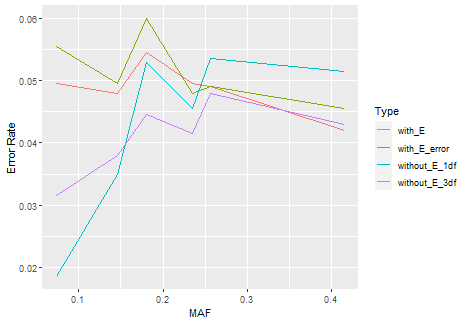
\includegraphics{stats-gene-research-progress-v9_files/figure-latex/unnamed-chunk-10-1.png}

Here we pick the last set of simulation (with the MAF of casual gene
being 0.42), and study the relationship between MAF and type I error
more closely:

\begin{Shaded}
\begin{Highlighting}[]
\NormalTok{all_error <-}\StringTok{ }\NormalTok{power}
\NormalTok{all_error}\OperatorTok{$}\NormalTok{MAF_level <-}\StringTok{ }\KeywordTok{ifelse}\NormalTok{(all_error}\OperatorTok{$}\NormalTok{MAF }\OperatorTok{>=}\StringTok{ }\FloatTok{0.1}\NormalTok{, }\StringTok{"0.1-0.15"}\NormalTok{,}\StringTok{"0.05-0.1"}\NormalTok{)}
\NormalTok{all_error}\OperatorTok{$}\NormalTok{MAF_level <-}\StringTok{ }\KeywordTok{ifelse}\NormalTok{(all_error}\OperatorTok{$}\NormalTok{MAF }\OperatorTok{>=}\StringTok{ }\FloatTok{0.15}\NormalTok{, }\StringTok{"0.15-0.2"}\NormalTok{, all_error}\OperatorTok{$}\NormalTok{MAF_level)}
\NormalTok{all_error}\OperatorTok{$}\NormalTok{MAF_level <-}\StringTok{ }\KeywordTok{ifelse}\NormalTok{(all_error}\OperatorTok{$}\NormalTok{MAF }\OperatorTok{>=}\StringTok{ }\FloatTok{0.2}\NormalTok{, }\StringTok{"0.2-0.25"}\NormalTok{, all_error}\OperatorTok{$}\NormalTok{MAF_level)}
\NormalTok{all_error}\OperatorTok{$}\NormalTok{MAF_level <-}\StringTok{ }\KeywordTok{ifelse}\NormalTok{(all_error}\OperatorTok{$}\NormalTok{MAF }\OperatorTok{>=}\StringTok{ }\FloatTok{0.25}\NormalTok{, }\StringTok{"0.25-0.3"}\NormalTok{, all_error}\OperatorTok{$}\NormalTok{MAF_level)}
\NormalTok{all_error}\OperatorTok{$}\NormalTok{MAF_level <-}\StringTok{ }\KeywordTok{ifelse}\NormalTok{(all_error}\OperatorTok{$}\NormalTok{MAF }\OperatorTok{>=}\StringTok{ }\FloatTok{0.3}\NormalTok{, }\StringTok{"0.3-0.5"}\NormalTok{, all_error}\OperatorTok{$}\NormalTok{MAF_level)}


\NormalTok{all_error <-}\StringTok{ }\NormalTok{all_error }\OperatorTok\StringTok{ }\KeywordTok{group_by}\NormalTok{(MAF_level) }\OperatorTok\StringTok{ }\KeywordTok{summarise}\NormalTok{(}\DataTypeTok{proposed_1 =} \KeywordTok{mean}\NormalTok{(proposed_}\DecValTok{1}\NormalTok{),}\DataTypeTok{proposed_2 =} \KeywordTok{mean}\NormalTok{(proposed_}\DecValTok{2}\NormalTok{), }\DataTypeTok{oracle =} \KeywordTok{mean}\NormalTok{(oracle), }\DataTypeTok{oracle_error =} \KeywordTok{mean}\NormalTok{(oracle_error), }\DataTypeTok{number =} \DecValTok{2000}\OperatorTok{*}\KeywordTok{n}\NormalTok{())}

\NormalTok{all_error <-}\StringTok{ }\NormalTok{all_error }\OperatorTok\StringTok{ }\KeywordTok{mutate}\NormalTok{(}\DataTypeTok{upper =} \FloatTok{0.05} \OperatorTok{+}\StringTok{ }\DecValTok{3}\OperatorTok{*}\KeywordTok{sqrt}\NormalTok{(}\FloatTok{0.05}\OperatorTok{*}\FloatTok{0.95}\OperatorTok{/}\NormalTok{number), }\DataTypeTok{lower =} \FloatTok{0.05} \OperatorTok{-}\StringTok{ }\DecValTok{3}\OperatorTok{*}\KeywordTok{sqrt}\NormalTok{(}\FloatTok{0.05}\OperatorTok{*}\FloatTok{0.95}\OperatorTok{/}\NormalTok{number))}

\NormalTok{all_error }\OperatorTok\StringTok{ }\KeywordTok{pivot_longer}\NormalTok{(proposed_}\DecValTok{1}\OperatorTok{:}\NormalTok{oracle_error, }\StringTok{"Type"}\NormalTok{, }\DataTypeTok{values_to =} \StringTok{"Error"}\NormalTok{) }\OperatorTok\StringTok{ }\KeywordTok{ggplot}\NormalTok{(}\KeywordTok{aes}\NormalTok{(}\KeywordTok{factor}\NormalTok{(MAF_level))) }\OperatorTok{+}\StringTok{ }\KeywordTok{geom_point}\NormalTok{(}\KeywordTok{aes}\NormalTok{(}\DataTypeTok{y =}\NormalTok{ Error, }\DataTypeTok{color =}\NormalTok{ Type), }\DataTypeTok{size =} \DecValTok{3}\NormalTok{, }\DataTypeTok{alpha =} \DecValTok{1}\NormalTok{) }\OperatorTok{+}\StringTok{ }\KeywordTok{geom_hline}\NormalTok{(}\KeywordTok{aes}\NormalTok{(}\DataTypeTok{yintercept =} \FloatTok{0.05}\NormalTok{)) }\OperatorTok{+}\StringTok{  }\KeywordTok{geom_pointrange}\NormalTok{(}\KeywordTok{aes}\NormalTok{(}\DataTypeTok{y =} \FloatTok{0.05}\NormalTok{, }\DataTypeTok{ymin =}\NormalTok{ lower, }\DataTypeTok{ymax =}\NormalTok{ upper), }\DataTypeTok{size =} \FloatTok{0.1}\NormalTok{)}
\end{Highlighting}
\end{Shaded}

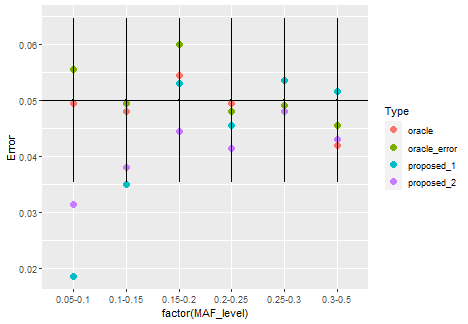
\includegraphics{stats-gene-research-progress-v9_files/figure-latex/unnamed-chunk-11-1.png}

\begin{Shaded}
\begin{Highlighting}[]
\NormalTok{all_error_plot <-}\StringTok{ }\NormalTok{all_error }\OperatorTok\StringTok{ }\KeywordTok{pivot_longer}\NormalTok{(proposed_}\DecValTok{1}\OperatorTok{:}\NormalTok{oracle_error, }\StringTok{"Type"}\NormalTok{, }\DataTypeTok{values_to =} \StringTok{"Error"}\NormalTok{) }\OperatorTok\StringTok{ }\KeywordTok{mutate}\NormalTok{(}\DataTypeTok{Type =} \KeywordTok{factor}\NormalTok{(Type))}
\KeywordTok{levels}\NormalTok{(all_error_plot}\OperatorTok{$}\NormalTok{Type) <-}\StringTok{ }\KeywordTok{c}\NormalTok{(}\StringTok{"with_E"}\NormalTok{,}\StringTok{"with_E_error"}\NormalTok{, }\StringTok{"without_E_1df"}\NormalTok{, }\StringTok{"without_E_3df"}\NormalTok{)}

\NormalTok{all_error_plot }\OperatorTok\StringTok{ }\KeywordTok{ggplot}\NormalTok{(}\KeywordTok{aes}\NormalTok{(}\KeywordTok{factor}\NormalTok{(MAF_level))) }\OperatorTok{+}\StringTok{ }\KeywordTok{geom_point}\NormalTok{(}\KeywordTok{aes}\NormalTok{(}\DataTypeTok{y =}\NormalTok{ Error, }\DataTypeTok{color =}\NormalTok{ Type), }\DataTypeTok{size =} \DecValTok{3}\NormalTok{) }\OperatorTok{+}\StringTok{ }\KeywordTok{geom_hline}\NormalTok{(}\KeywordTok{aes}\NormalTok{(}\DataTypeTok{yintercept =} \FloatTok{0.05}\NormalTok{)) }\OperatorTok{+}\StringTok{  }\KeywordTok{geom_pointrange}\NormalTok{(}\KeywordTok{aes}\NormalTok{(}\DataTypeTok{y =} \FloatTok{0.05}\NormalTok{, }\DataTypeTok{ymin =}\NormalTok{ lower, }\DataTypeTok{ymax =}\NormalTok{ upper), }\DataTypeTok{size =} \FloatTok{0.1}\NormalTok{)}
\end{Highlighting}
\end{Shaded}

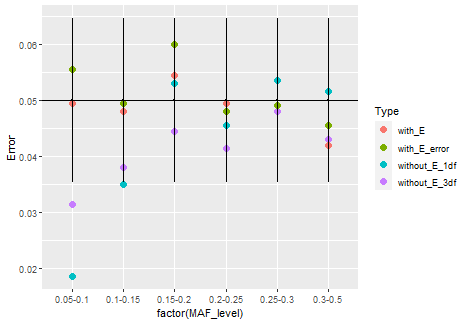
\includegraphics{stats-gene-research-progress-v9_files/figure-latex/unnamed-chunk-11-2.png}

Based on the above plot, all the procedures have type I error rate in
the expected range, when the MAF level is larger than 0.1.

\end{document}
